\documentclass{article}

\usepackage{arxiv}

\usepackage[utf8]{inputenc} % allow utf-8 input
\usepackage[T1]{fontenc}    % use 8-bit T1 fonts
\usepackage{lmodern}        % https://github.com/rstudio/rticles/issues/343
\usepackage{hyperref}       % hyperlinks
\usepackage{url}            % simple URL typesetting
\usepackage{booktabs}       % professional-quality tables
\usepackage{amsfonts}       % blackboard math symbols
\usepackage{nicefrac}       % compact symbols for 1/2, etc.
\usepackage{microtype}      % microtypography
\usepackage{lipsum}
\usepackage{graphicx}

\title{Optimal amount of gut content data required to predict trophic
interactions using a food web model}

\author{
    Anubhav Gupta
    \thanks{Corresponding author}
   \\
    Department of Evolutionary Biology and Environmental Studies \\
    University of Zurich \\
  8057 Zurich, Switzerland \\
  \texttt{\href{mailto:anubhav.gupta@ieu.uzh.ch}{\nolinkurl{anubhav.gupta@ieu.uzh.ch}}} \\
   \And
    Eoin O' Gorman
   \\
    School of Life Sciences \\
    University of Essex \\
  CO4 3SQ Colchester, UK \\
  \texttt{\href{mailto:e.ogorman@essex.ac.uk}{\nolinkurl{e.ogorman@essex.ac.uk}}} \\
   \And
    Owen L. Petchey
   \\
    Department of Evolutionary Biology and Environmental Studies \\
    University of Zurich \\
  8057 Zurich, Switzerland \\
  \texttt{\href{mailto:owen.petchey@ieu.uzh.ch}{\nolinkurl{owen.petchey@ieu.uzh.ch}}} \\
  }


% Pandoc citation processing
\newlength{\csllabelwidth}
\setlength{\csllabelwidth}{3em}
\newlength{\cslhangindent}
\setlength{\cslhangindent}{1.5em}
% for Pandoc 2.8 to 2.10.1
\newenvironment{cslreferences}%
  {}%
  {\par}
% For Pandoc 2.11+
\newenvironment{CSLReferences}[3] % #1 hanging-ident, #2 entry spacing
 {% don't indent paragraphs
  \setlength{\parindent}{0pt}
  % turn on hanging indent if param 1 is 1
  \ifodd #1 \everypar{\setlength{\hangindent}{\cslhangindent}}\ignorespaces\fi
  % set entry spacing
  \ifnum #2 > 0
  \setlength{\parskip}{#2\baselineskip}
  \fi
 }%
 {}
\usepackage{calc} % for calculating minipage widths
\newcommand{\CSLBlock}[1]{#1\hfill\break}
\newcommand{\CSLLeftMargin}[1]{\parbox[t]{\csllabelwidth}{#1}}
\newcommand{\CSLRightInline}[1]{\parbox[t]{\linewidth - \csllabelwidth}{#1}}
\newcommand{\CSLIndent}[1]{\hspace{\cslhangindent}#1}

\usepackage{lineno}
\linenumbers
\usepackage {amsmath}
\setlength\parindent{24pt}
\usepackage{setspace}\doublespacing


\begin{document}
\maketitle

\def\tightlist{}


\begin{abstract}
\begin{enumerate}
\def\labelenumi{\arabic{enumi})}
\tightlist
\item
\item
\item
\item
\end{enumerate}
\end{abstract}

\keywords{
    gut content data
   \and
    ADBM
   \and
    food web accuracy
   \and
    food web prediction
  }

\hypertarget{alternate-titles}{%
\section{Alternate titles}\label{alternate-titles}}

\begin{itemize}
\item
  Predicting trophic interactions using incomplete gut content data
\item
  Effect of the amount of gut content data on the accuracy and precision
  of food web prediction
\end{itemize}

\hypertarget{introduction}{%
\section{Introduction}\label{introduction}}

Knowledge about the trophic interactions in a food web is crucial in
ecology from identifying keystone species (Jord'an 2009) to quantifying
robustness of a food web to species extinctions (Dunne, Williams, and
Martinez 2002). This has led to the development of numerous food web
models (Allesina, Alonso, and Pascual 2008; Cohen, Newman, and Steele
1985; Gravel et al. 2013; Petchey et al. 2008; Tamaddoni-Nezhad et al.
2013). Along with inferring missing links in an observed food web, the
food web models are also used for ecological forecasting (Hattab et al.
2016; Lindegren et al. 2010) and understanding the underlying mechanism
governing the interactions in a food web (O'NAGorman et al. 2019).

Although food web models are constructed using prior theory governing
the food webs, interaction data is required to parameterise a model. For
example, Petchey et al. (2008) used presence-absence information about
trophic interactions to parameterise the allometric diet breadth model
and thereby predict species interactions. These information can be
inferred from diverse set of methods such as gut content analysis
(Peralta-Maraver, Lopez-Rodriguez, and de Figueroa 2017), stable isotope
ratio analysis of tissues (Layman et al. 2007), experimentation (Warren
1989), DNA metabarcoding (Roslin and Majaneva 2016) and literature
research (Gray et al. 2015; Cohen and Mulder 2014; Goldwasser and
Roughgarden 1993). All of these methods can infer the diet of a
consumer, however different methods measure different consumed
components, thereby resulting in different levels of uncertainty in the
inferred diet (citreqd). A single gut content of a predator describes
what that individual has consumed recently which can be used to infer
the diet of the predator (Eitzinger et al. 2018; O'NAMalley et al. 2017;
Dixon et al. 2017; McClain-Counts, Demopoulos, and Ross 2017;
Peralta-Maraver, Lopez-Rodriguez, and de Figueroa 2017). Stable isotope
data when combined with mixing models can be used to determine which
prey items are most likely fed upon by a predator (Kadoya, Osada, and
Takimoto 2012; Crawford, Mcdonald, and Bearhop 2008).

Acquiring food web data from these methods is time consuming and
expensive (reference). For example, many gut content data needs to be
collected to infer the complete presence-absence information of a food
web structure with high accuracy and precision. Also further time and
resource investment is required to process the collected samples. Hence,
there is an utmost demand to know the minimum number of presence-absence
information of a food web to parameterise a food web model with high
accuracy and high precision, so that one knows when to stop collecting
any further data on the food web.

The key question we are interested in answering is how much
presence-absence information is required to infer food web structure
from a food web model with high accuracy and high precision. In other
words, in case of gut content data how many samples of gut content
should one collect from the field to parameterise a food web model? To
answer this question, we use the presence-absence information from gut
content data, and allometric diet breadth model (ADBM) to predict
trophic interactions. We parameterise the model using approximate
Bayesian computation/rejection Monte Carlo sampling.

\hypertarget{materials-and-methods}{%
\section{Materials and Methods}\label{materials-and-methods}}

In the upcoming sections, we present the allometric diet breadth model
(ADBM) and the gut content data used to infer trophic interactions. We
also give a detailed account of using partial gut content data to
parameterise the ADBM using approximate Bayesian computation (ABC). We
assessed model predictions using true skill statistic and various
structural food web properties for comparison across food webs.

\hypertarget{allometric-diet-breadth-model-adbm}{%
\subsection{Allometric Diet Breadth Model
(ADBM)}\label{allometric-diet-breadth-model-adbm}}

The allometric diet breadth model (ADBM) is based on optimal foraging
theory, specifically the contingency foraging model (MacArthur and
Pianka 1966). The ADBM predicts the set of prey species a consumer
should feed upon to maximise its rate of energy intake (Petchey et al.
2008). The foraging variables in the model: energy content of the
resources, handling times of the prey, space clearance rate and prey
densities are allometrically scaled to the body sizes of the species.

\hypertarget{broadstone-stream}{%
\subsection{Broadstone Stream}\label{broadstone-stream}}

Broadstone Stream (51\(^\circ\) 05' N 0\(^\circ\) 03' E; 120 m above
sea-level) is a second-order tributary of the River Medway in south-east
England. It is dominated by invertebrates as the acidity of the stream
(pH 4.7-6.6) excludes fish. The stream consists of 25 common
invertebrate species (Woodward, Speirs, and Hildrew 2005a). Among the
predators, the three large species are \emph{Cordulegaster boltonii}
Donovan, \emph{Sialis fuliginosa} Pict. and \emph{Plectrocnemia
conspersa} {[}Curtis{]} and the three small species are the larvae of
the tanypod midges \emph{Macropelopia nebulosa} {[}Meigen{]},
\emph{Trissopelopia longimana} {[}Staeger{]}, and \emph{Zavrelimyia
barbatipes} {[}Kieffer{]}. Broadstone Stream food web is one of the most
completely described food webs available for any system (J. M.
Schmid-Araya et al. 2002; Hildrew 2009; Layer et al. 2010; and Woodward,
Speirs, and Hildrew 2005b).

\hypertarget{celtic-sea}{%
\subsection{Celtic Sea}\label{celtic-sea}}

The Celtic Sea is an area of continental shelf bordered by Ireland, the
UK and the Bay of Biscay. Precise sampling locations and dates were not
given in the Barnes et al.~(2008) dataset, from where the data used in
this chapter were extracted, so we pooled data over the whole time
period and locations to capture general patterns. Only locations
consistently sampled through the 1987--2001 time series were used
(Blanchard et al., 2005).

The feeding links of fishes in the Celtic Sea have been described in a
published global dataset of individual predator and prey body sizes and
taxonomy (Barnes et al., 2008): in total, 1988 feeding events from 29
predator species were included in the food web presented here. The
original stomach contents data were collected from dissections carried
out on board research vessels during the annual surveys carried out by
the Centre for Environment, Fisheries and Aquaculture Science (Cefas)
(Pinnegar et al., 2003). Predator and prey length were recorded and
converted to body mass by Barnes et al.~(2008) using published
regression equations. Only vertebrate prey were identified and measured,
with the vast majority being identified to species.

\hypertarget{afon-hirnant}{%
\subsection{Afon Hirnant}\label{afon-hirnant}}

The Afon Hirnant is a tributary of the Welsh Dee in North Wales, U.K.
(52\(^\circ\) 52'N 03\(^\circ\) 34) with the study being conducted at
three sites. The pH within each site ranged from about 5.5 to 7 over the
course of the year.

A total of 180 invertebrate samples were collected for the whole
sampling periods. All individuals within the benthic samples were
counted and identified to the lowest possible taxonomic level (usually
species). Prey items were identified using a combination of taxonomic
keys and reference slides of previously identified species, after Jenny
M. Schmid-Araya et al. (2002); J. M. Schmid-Araya et al. (2002).

\hypertarget{tadnoll-brook}{%
\subsection{Tadnoll Brook}\label{tadnoll-brook}}

Description of Tadnoll Brook here

\hypertarget{coilaco}{%
\subsection{Coilaco}\label{coilaco}}

Description of Coilaco here

\hypertarget{guampoe}{%
\subsection{Guampoe}\label{guampoe}}

Description of Guampoe here

\hypertarget{trancura}{%
\subsection{Trancura}\label{trancura}}

Description of Trancura here

\hypertarget{food-web-construction}{%
\subsection{Food web construction}\label{food-web-construction}}

Presence and absence interactions of food web data can be aggregated in
different ways (Gilljam et al. 2011). A common way of aggregating food
web data is the taxonomic approach, where a species is defined as
predating on another if at least one prey species individual was found
in the gut of a predator species individual. Whereas in size-class food
web, a feeding link was assigned if at least one prey item within a size
class was found in the gut of a predator of another size class,
irrespective of their taxonomy. In our study, we aggregate the food web
on the basis of size class.

\hypertarget{assessment-of-prediction}{%
\subsection{Assessment of prediction}\label{assessment-of-prediction}}

The accuracy of the predicted diet of the predators was defined using
true skill statistic (TSS) which takes into account the true and false
predictions of both the presence and absence of links defined as:

\[ \text{TSS} = \frac{ad-bc}{(a+c)(b+d)} \] where \(a\) is the number of
observed links that are predicted by the model (true positives), \(d\)
is the number of observed absences of links that are correctly predicted
(true negatives), \(b\) is the number of false positives, and \(c\) is
the number of false negatives.

The \(TSS\) ranges from \(-1\) to \(1\), where +1 indicates a perfect
prediction. A \(TSS\) value of zero or less indicates a performance no
better than random (Allouche, Tsoar, and Kadmon 2006).

\hypertarget{inferring-food-web-using-partial-gut-content-data}{%
\subsection{Inferring food web using partial gut content
data}\label{inferring-food-web-using-partial-gut-content-data}}

From a pool of gut content data, we draw a set of gut content data
randomly. Then we used the rejection ABC to accept a parameter value
from a prior distribution which would have resulted in the minimum
distance, where distance = 1 - True skill statistic. The true skill
statistic was computed between the predators' diet predicted from the
ADBM, and that from the sampled gut content data. We repeated this
process for \(n~(= 100)\) number of times for every \(i\) number of
guts, where \(i\) lies between 1 and total number of gut content data in
the pool.

\emph{Input:}

\begin{itemize}
\item
  Predators \(P: P = \{p_1, p_2, \dots, p_k \}\)
\item
  A pool of gut content data \(G: G = \{g_1, g_2, \dots, g_n\}\), where
  \(g_{n}\) is a one-dimensional matrix containing ones and zeros.
\item
  A model prediction
  \(model(\theta): ADBM(\theta) = \{d_{p_1}, d_{p_1}, \dots, d_{p_k}\}\),
  where \(d_{p_k}\) is a one-dimensional diet matrix of predator \(k\)
  containing ones and zeros.
\item
  A summary statistic \(s(x): s(x) \subseteq model(\theta)\)
\item
  A distance function \(d(x_i, y) : d(x_i,y) = 1 - TSS(x_i, y)\)
\item
  An observed food web
  \(Y: Y = \{d_{p_1}', d_{p_1}', \dots, d_{p_k}'\}\)
\end{itemize}

\emph{Sampling:}

for \(i = 1, \dots, tgut\) where \(tgut\) is the total number of gut
content data in the pool \(G\)

\begin{itemize}
\item
  for \(j = 1, \dots, nsample\) where \(nsample\) is the number of
  independent samples to be drawn

  \begin{itemize}
  \item
    Draw a set of gut content data \(y = \{g_1, g_2, \dots, g_i\}\) from
    the pool of gut content data \(G\)
  \item
    for \(k = 1, \dots, npar\) where \(npar\) is the number of parameter
    values to be sampled

    \begin{itemize}
    \item
      Draw a set of parameter values \(\theta_k\) from the prior
      distribution \(\pi(\theta)\)
    \item
      Compute the model result \(x_i = model(\theta_k)\)
    \item
      Compute \(s(x_i)\) and \(d(s(x_i), y)\)
    \end{itemize}
  \item
    Accept \(\theta_j\), which results in the \(min_i\{d(s(x_i), y)\}\)
  \end{itemize}
\item
  Compute
  \(TSS_{i}(x, y) = \{TSS(x_i,y): x_i = ADBM(\theta_j), \theta_j \text{ computed from previous step}\}\)
  using the accepted \(\theta_1, \dots, \theta_{nsample}\)
\end{itemize}

\emph{Output:}

A prediction interval containing \(TSS\) between observed and predicted
food webs for every \(i\) number of gut content data drawn from the pool
of gut content data.

\hypertarget{results}{%
\section{Results}\label{results}}

We first present how the accuracy of the food web model vary in
predicting trophic interactions when we increase the amount the gut
content data provided to the food web model. Then, we calculate the
number of gut content data for each food webs corresponding to which the
accuracy results in 90\% of the maximum true skill statistics predicted
by the food web model. We also compute the goodness of the food web
model in predicting structural properties from incomplete gut content
data. We did that by computing mean standardised error in food web
properties.

\hypertarget{inferring-trophic-interactions-using-adbm-and-incomplete-gut-content-data}{%
\subsection{Inferring trophic interactions using ADBM and incomplete gut
content
data}\label{inferring-trophic-interactions-using-adbm-and-incomplete-gut-content-data}}

\begin{figure}

{\centering 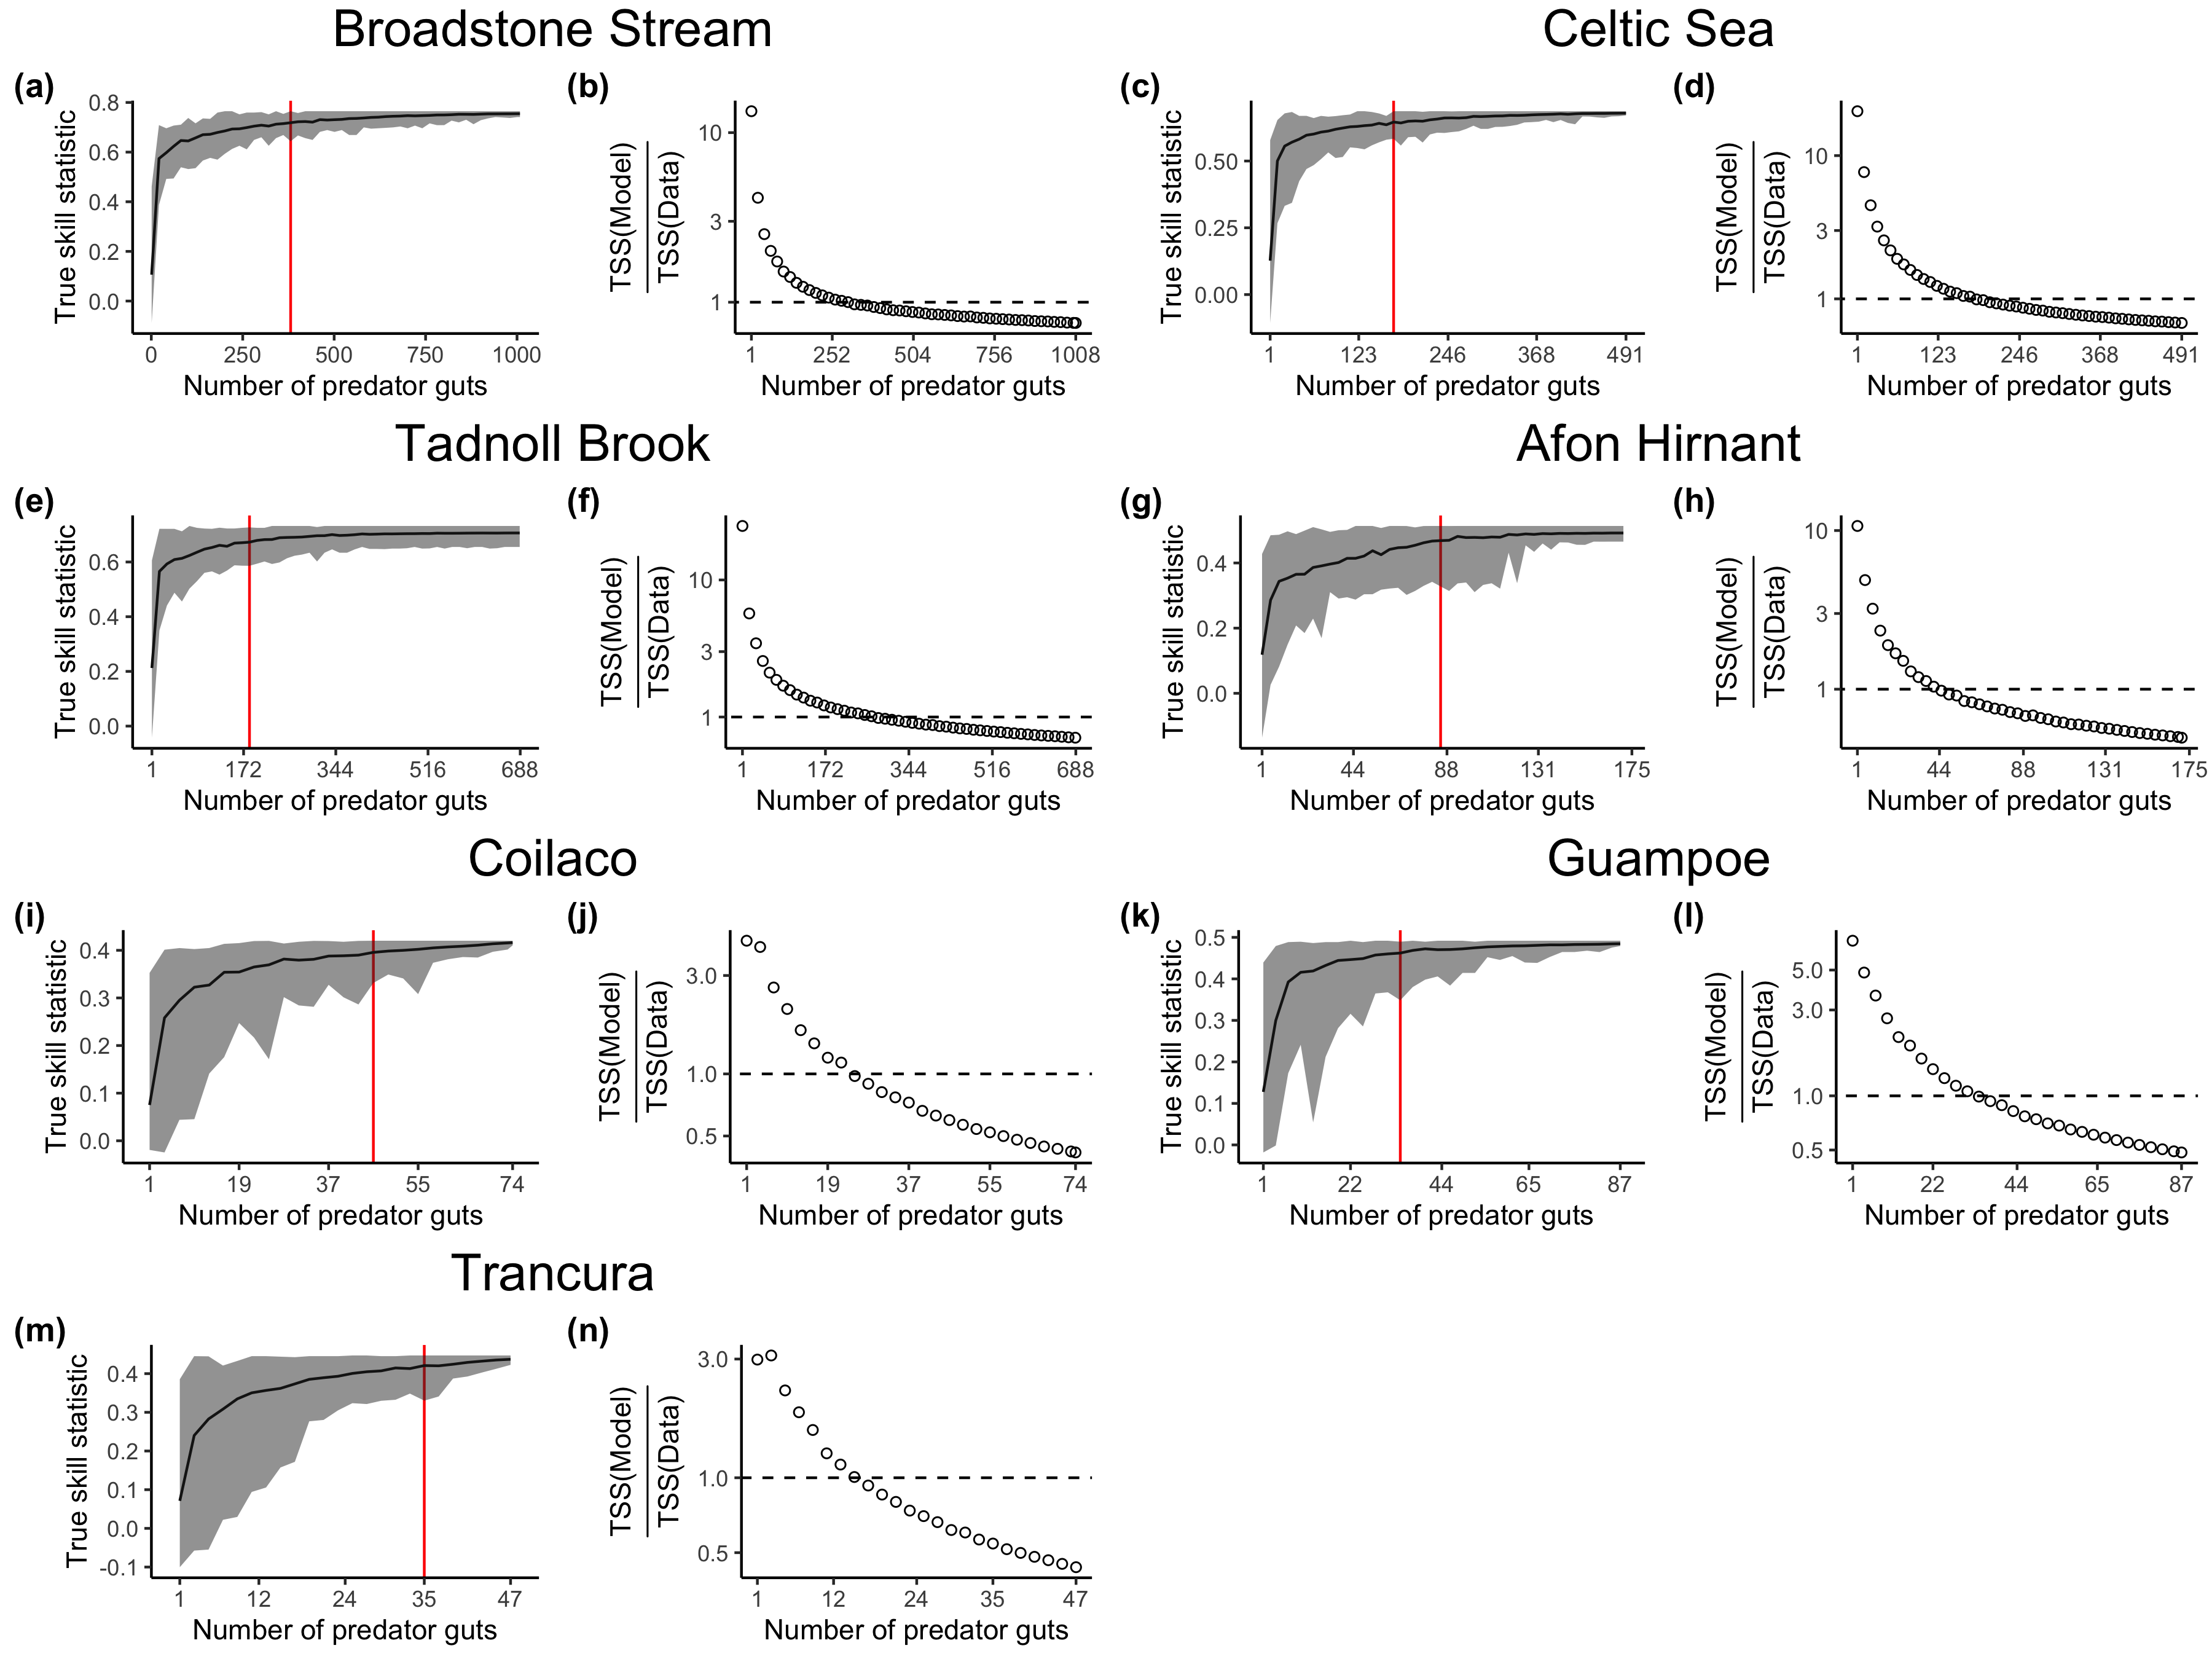
\includegraphics[width=500px]{../../results/misc/plot_TSS_ratio} 

}

\caption{\label{fig:fig_ra} (a, c, e, g, i, k, m) Accuracy of the predicted food web measured using the true skill statistics, predicted by the ADBM parameterised using gut content data. Line and shaded grey region represents the mean and the prediction interval of 100 independent samples respectively. Red line represents the number of predator guts required to achieve a TSS of 95\% of the maximum TSS. (b, d, f, h, j, l, n) Ratio of the true skill statistic of the predicted food web by the ADBM parameterised using gut content data to that of the predicted food web constructed using gut content data only. The dashed line shows where the ratio is one for reference.}\label{fig:unnamed-chunk-2}
\end{figure}

The true skill statistics of the food webs predicted by the ADBM using
subsets of gut content data improved quickly for lower number of
predator guts (Fig. \ref{fig:fig_ra}) (a, c, e, g, i, k, m). The
prediction interval of the true skill statistics reduced with the
increasing number of predator guts with the mean TSS asymptoting to the
maximum mean TSS achieved by the ADBM when all the gut content data was
used. Although the maximum TSS varied among the food webs, the
qualitative increase in the TSS was the same.

For a low number of predator guts, the TSS of the model predicted food
web was higher compared to the TSS of the food web constructed from gut
content data (Fig. \ref{fig:fig_ra} (b, d, f, h, j, l, n)), recommending
when a model can be used to compensate for undersampled links. After a
certain increase in the number of predator guts, the ratio
TSS(Model)/TSS(data) reduced to less than one, and reduced further
gradually.

With only 381 number of gut content data which is 38\% of the total gut
content data, the ADBM predicted the food web with TSS of 0.74 which was
95\% of the mean TSS (0.78) achieved using complete gut content data by
the ADBM for Broadstone Stream food web (Fig. \ref{fig:fig_ra}(a)). In
the case of the Celtic Sea food web, only 171 gut content data was
required by the ADBM to predict food web with TSS equal to 95\% of the
mean TSS (0.68) achieved using complete gut content data by the ADBM
(Fig. \ref{fig:fig_ra}(c)).

\hypertarget{dependence-of-minimum-gut-content-data-on-number-of-species-links-and-connectance}{%
\subsection{Dependence of minimum gut content data on number of species,
links and
connectance}\label{dependence-of-minimum-gut-content-data-on-number-of-species-links-and-connectance}}

There seems to be a positive relationship between number of minimum gut
content data and number of species (S) (Fig. \ref{fig:fig_rb} (a)),
links (L) (Fig. \ref{fig:fig_rb} (c)), connectance (C) (Fig.
\ref{fig:fig_rb} (d)) and number of predator nodes (Fig.
\ref{fig:fig_rb} (e)), with Broadstone Stream being an outlier in Fig.
\ref{fig:fig_rb} (a, c, e). The number of minimum gut content data
increases with number of maximum gut content data sampled (Fig.
\ref{fig:fig_rb} (b)). There seems to be a negative relationship between
proportion of minimum gut (= Number of minimum gut / Number of maximum
guts sampled) and number of species (S) (Fig. \ref{fig:fig_rb} (f)),
links (L) (Fig. \ref{fig:fig_rb} (g)), connectance (C) (Fig.
\ref{fig:fig_rb} (h)).

\begin{figure}

{\centering 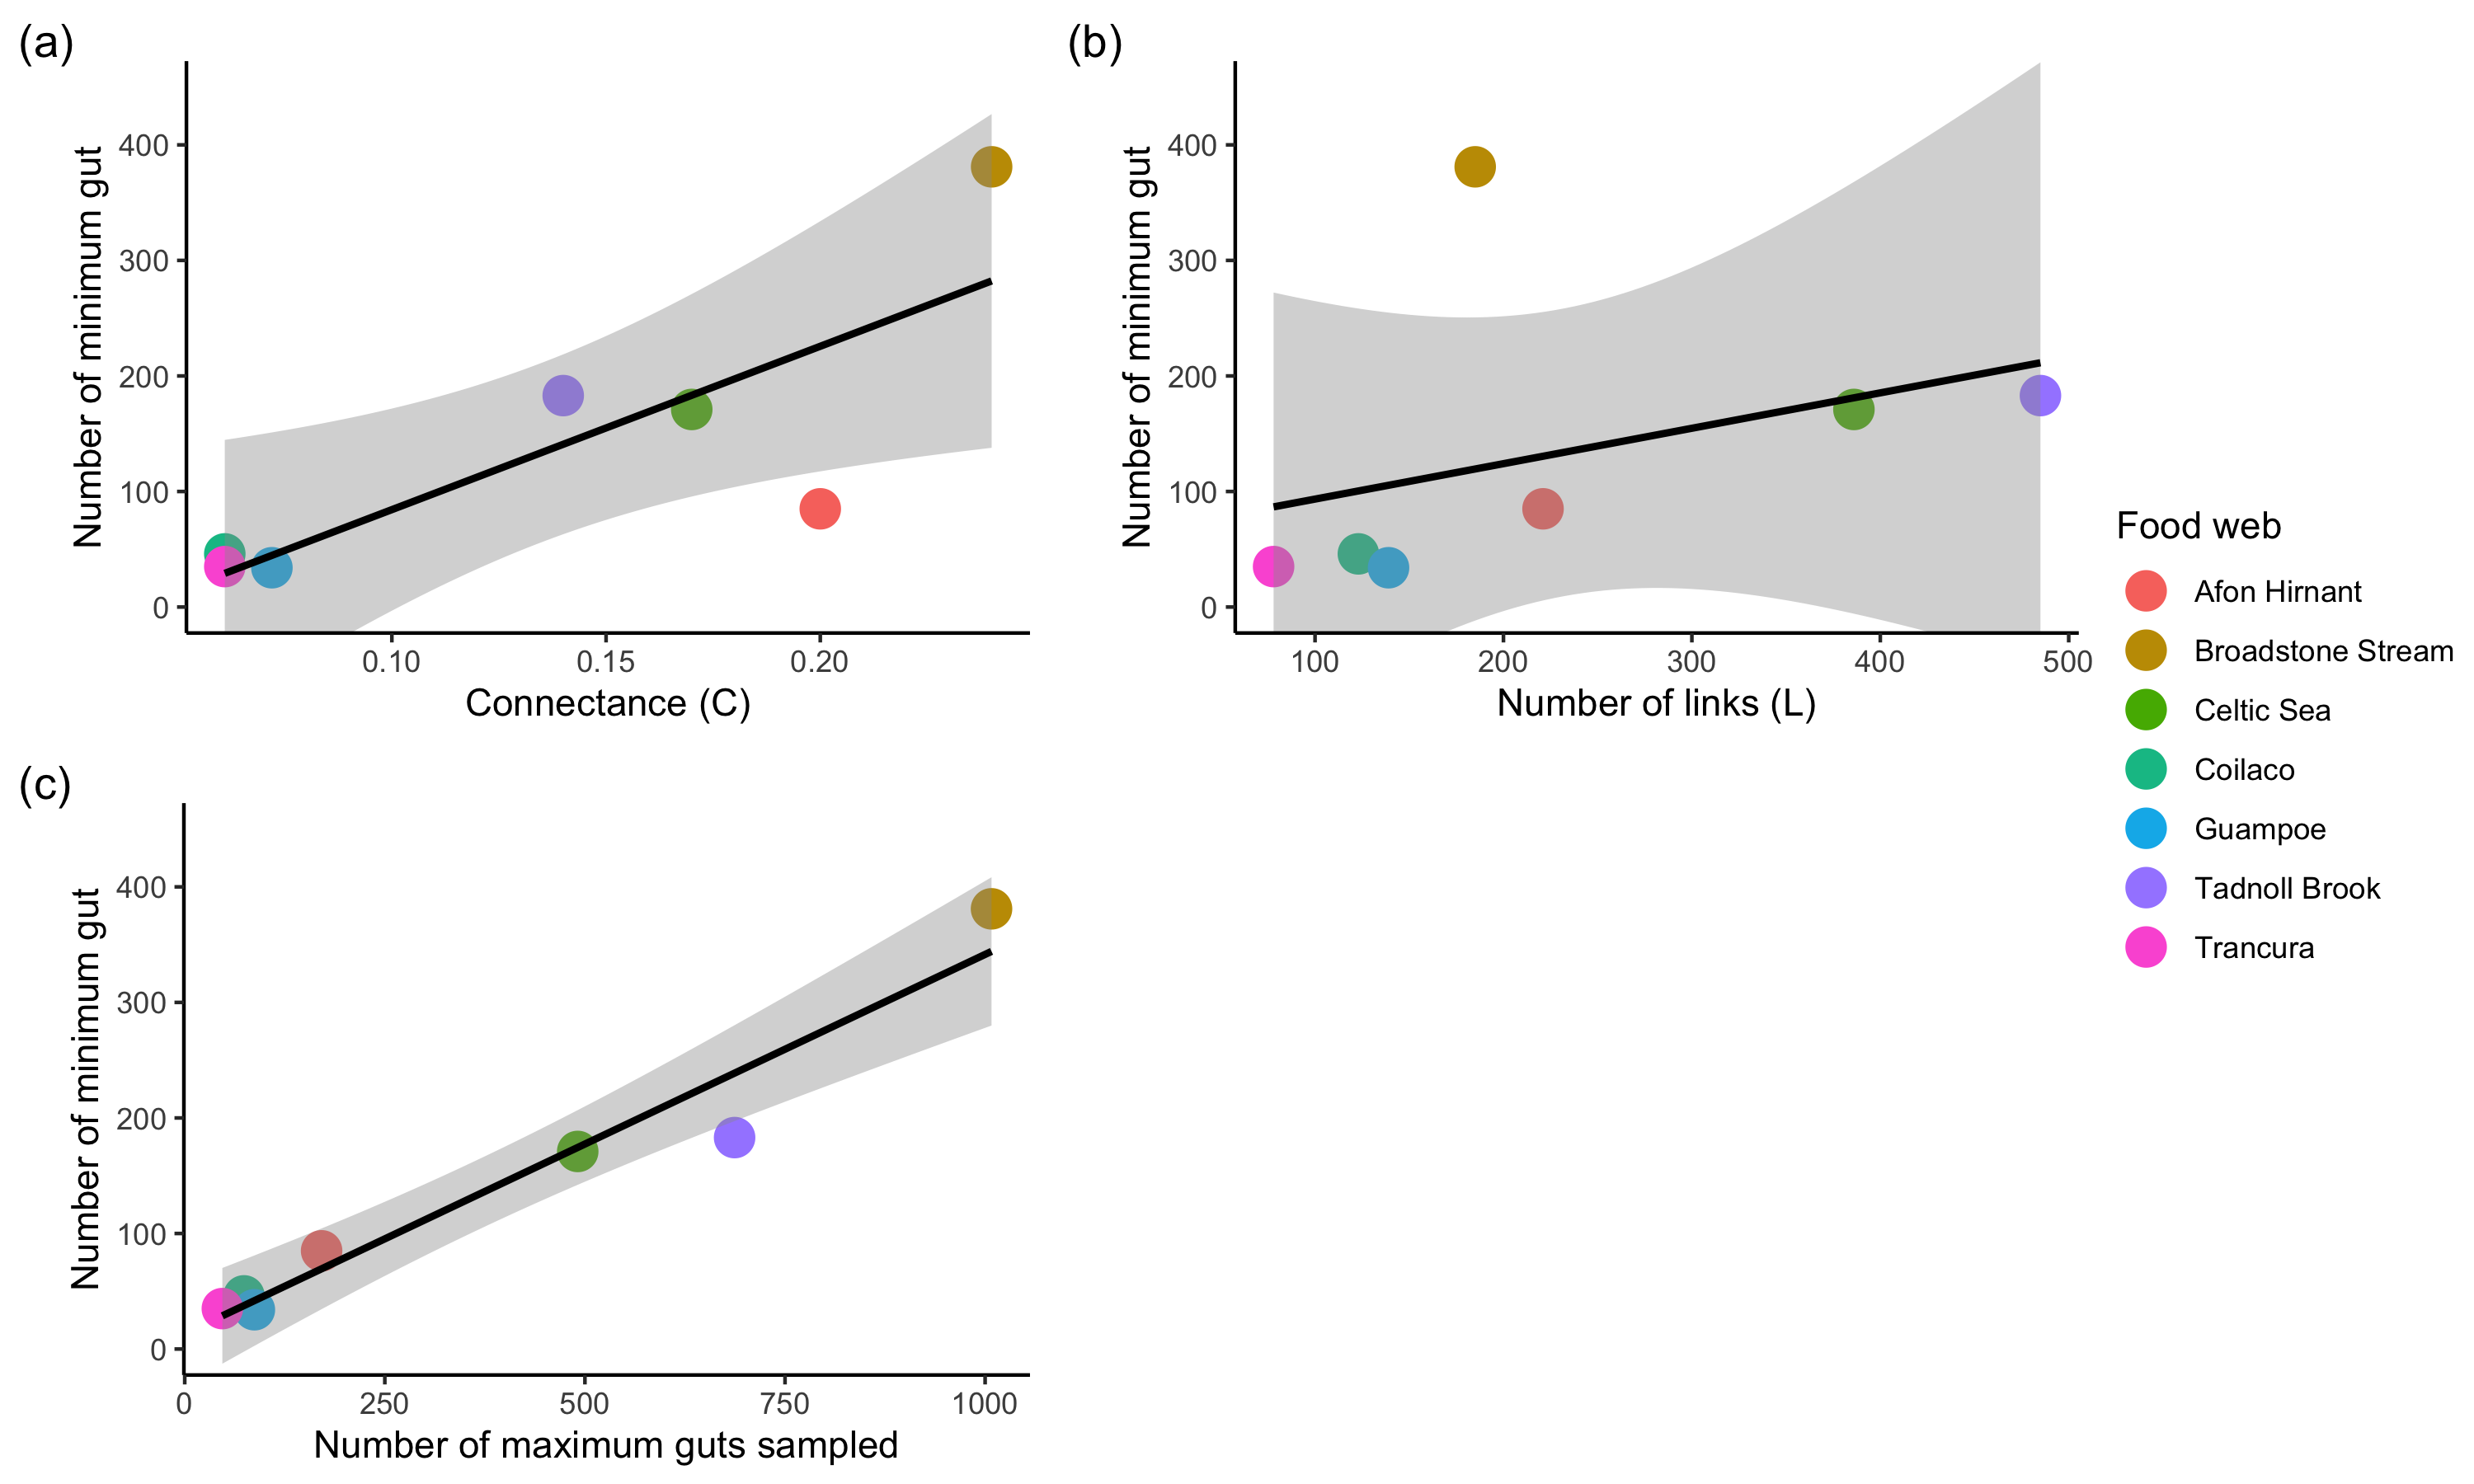
\includegraphics[width=500px]{../../results/misc/plot_min_gut_vs_X} 

}

\caption{\label{fig:fig_rb} (a, b, c, d, e) Number of minimum gut content data plotted against number of species (S), number of maximum guts sampled, number of links (L), connectance (C) and number of predator nodes respectively. (f, g, h) Proportion of minimum gut content data plotted against number of species (S), number of links (L) and connectance (C) respectively.}\label{fig:unnamed-chunk-3}
\end{figure}

\begin{figure}

{\centering 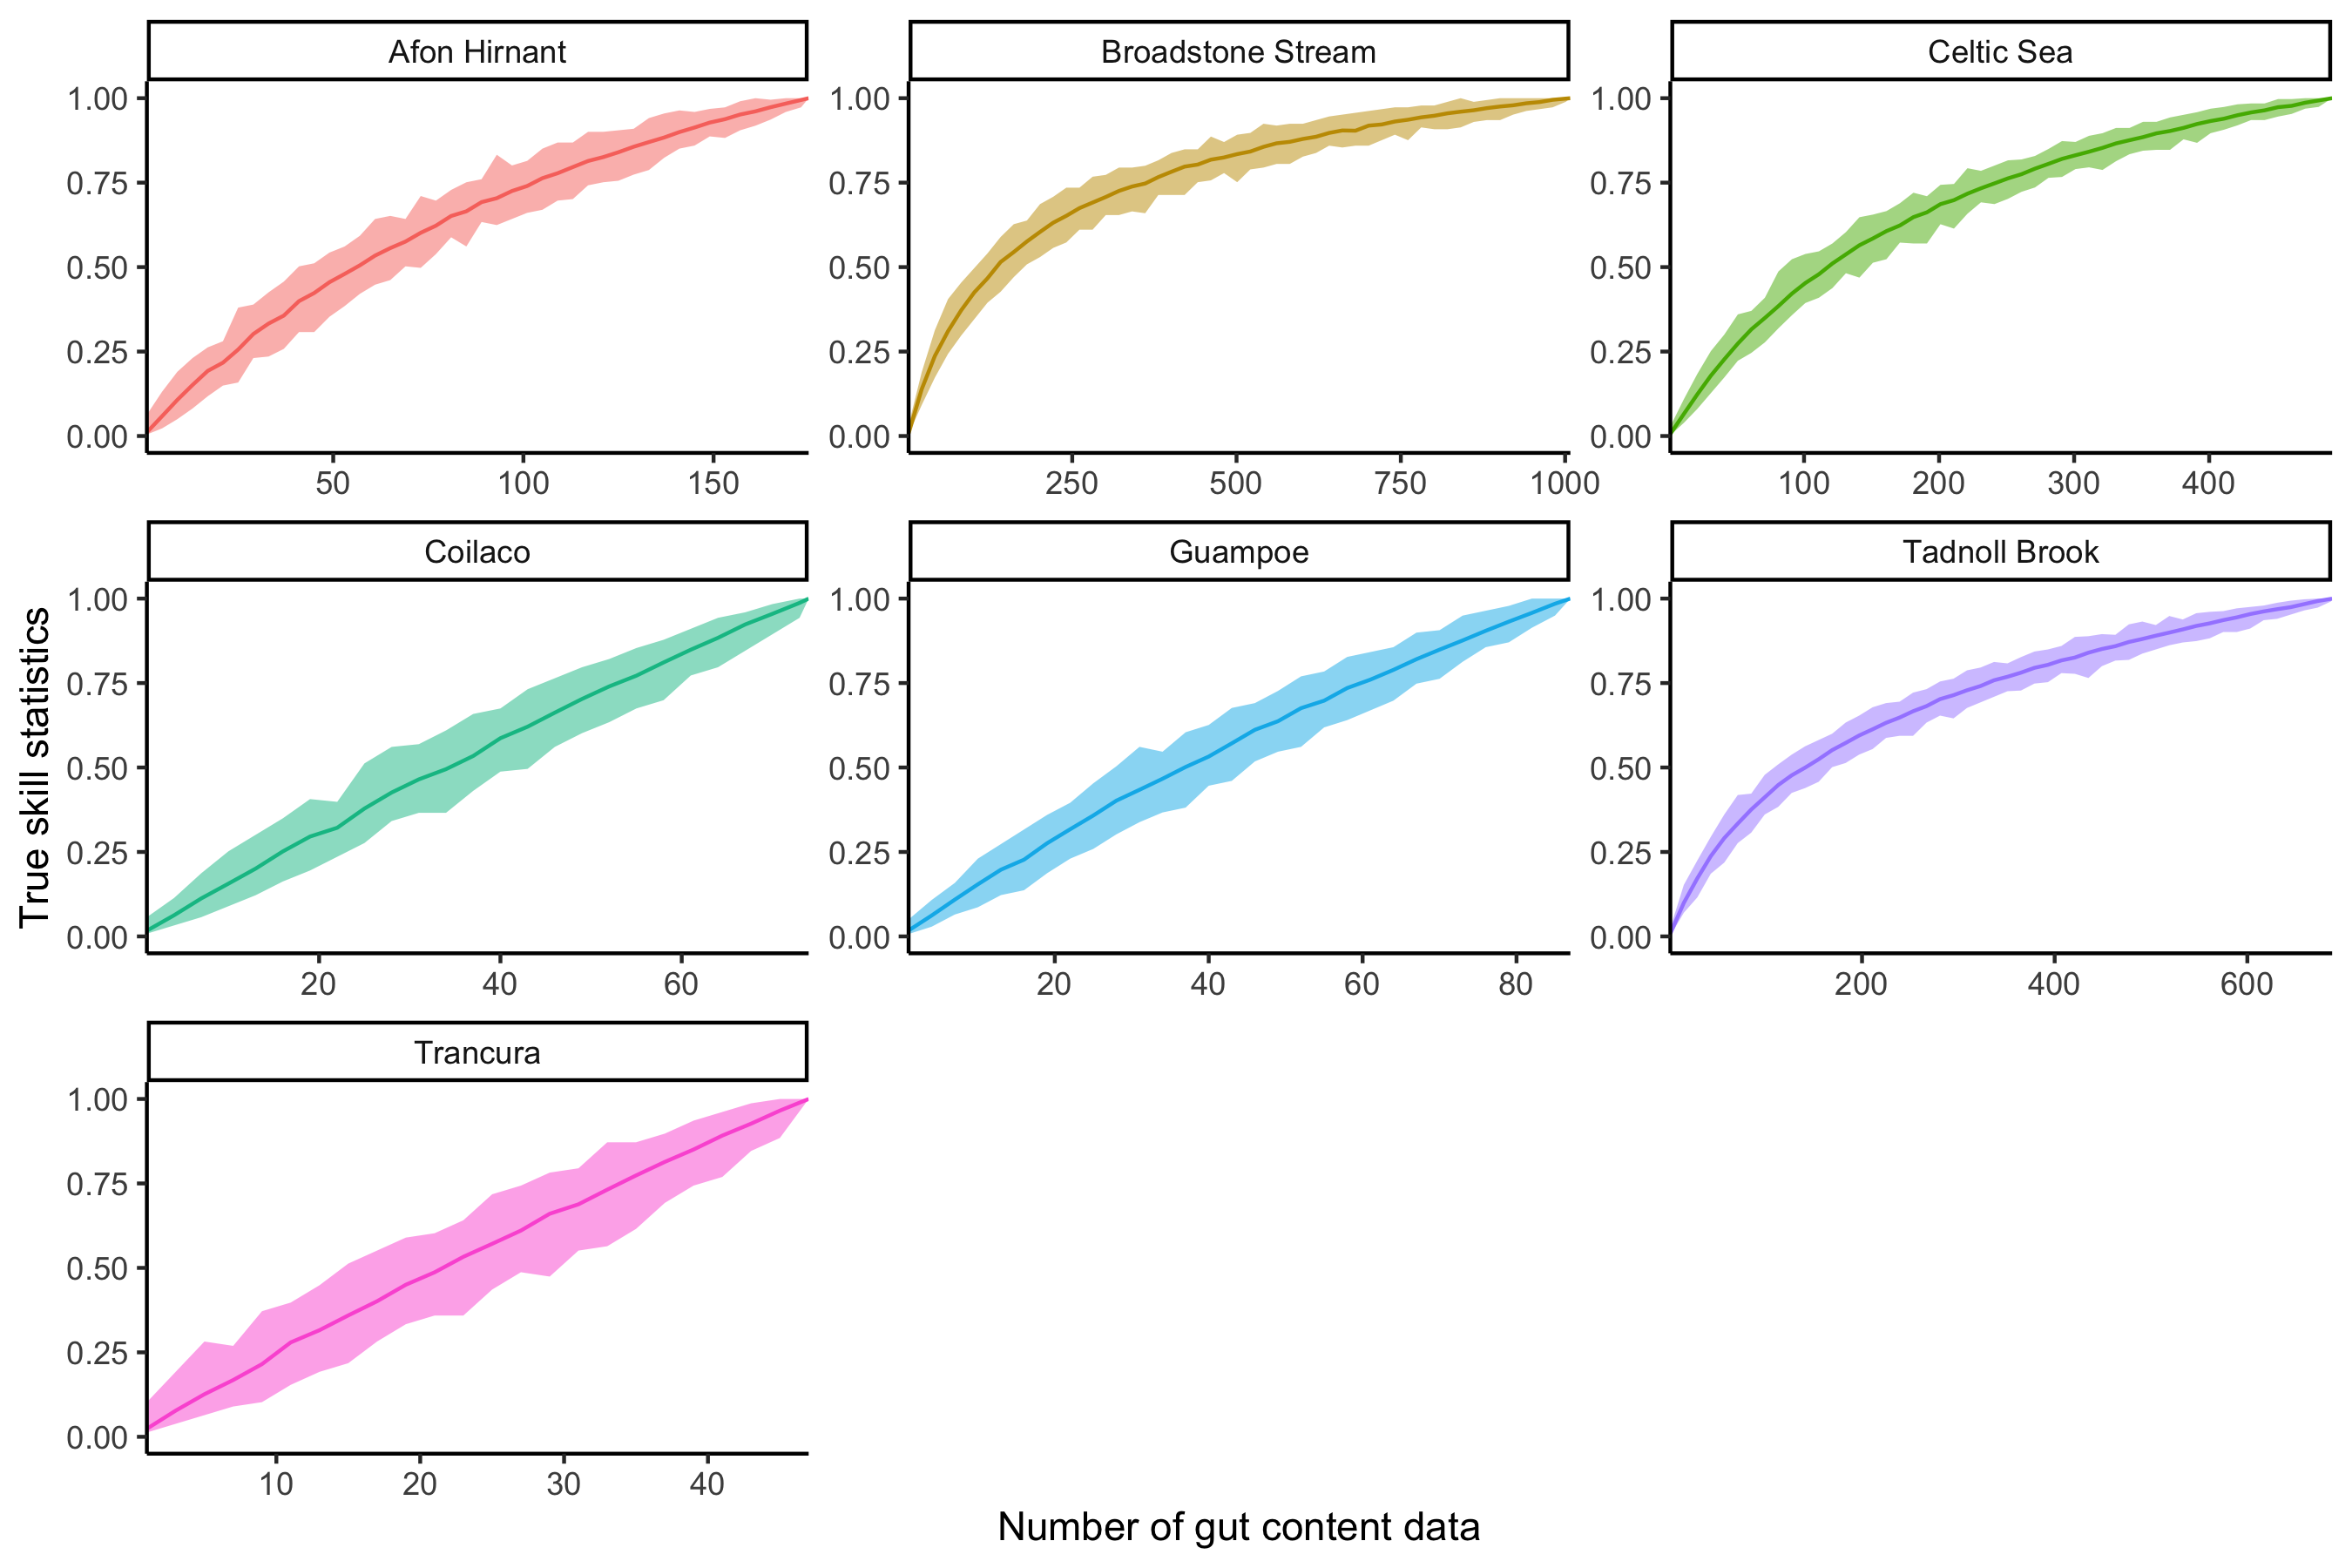
\includegraphics[width=500px]{../../results/misc/plot_empTSS_ngut} 

}

\caption{\label{fig:fig_rc} True skill statistics of the food web constructed using gut content data plotted against number of gut content data.}\label{fig:unnamed-chunk-4}
\end{figure}

\hypertarget{discussion}{%
\section{Discussion}\label{discussion}}

\hypertarget{why-broadstone-stream-is-an-outlier}{%
\subsection{Why Broadstone Stream is an
outlier?}\label{why-broadstone-stream-is-an-outlier}}

Broadstone Stream is the most sampled food web compared to all the other
food webs (Fig. \ref{fig:fig_rc}), which means the observed Broadstone
Stream food web might be more accurate compared to others.

\hypertarget{why-incomplete-gut-content-data-can-be-used-to-infer-trophic-interactions}{%
\subsection{Why incomplete gut content data can be used to infer trophic
interactions?}\label{why-incomplete-gut-content-data-can-be-used-to-infer-trophic-interactions}}

\begin{itemize}
\item
  Model fills up the missing interactions
\item
  Partial data helps to constrain the parameter space
\end{itemize}

\hypertarget{there-is-uncertainty-in-gut-content-data-and-needs-to-be-propagated-into-models-predictions}{%
\subsection{There is uncertainty in gut content data and needs to be
propagated into model's
predictions}\label{there-is-uncertainty-in-gut-content-data-and-needs-to-be-propagated-into-models-predictions}}

There is considerable uncertainty involved in gut content analysis
(Baker, Buckland, and Sheaves 2014) such as in fish's guts, there are
sometimes loose tissues that are not identifiable and cannot be assigned
to a specific prey item with certainty. There are factors such as sample
size of consumers, mechanical prey handling, differential digestion and
evacuation rates of different prey types and volumes, and the ingestion
order that in combination result in an unquantifiable error which is
difficult to interpret in the predator diet (Hyslop 1980; Rindorf and
Lewy 2004; Baker, Buckland, and Sheaves 2014). Therefore, a future
development would be to consider how this uncertainty is propagated into
food web prediction.

\hypertarget{comparing-our-study-with-other-studies-of-predicting-food-webs-using-incomplete-data}{%
\subsection{Comparing our study with other studies of predicting food
webs using incomplete
data}\label{comparing-our-study-with-other-studies-of-predicting-food-webs-using-incomplete-data}}

Some studies have presented how the accuracy of food web prediction
change when we vary the amount of food web data (Gray et al. 2015).

\hypertarget{what-is-the-generalisability-of-our-results}{%
\subsection{What is the generalisability of our
results?}\label{what-is-the-generalisability-of-our-results}}

\begin{itemize}
\tightlist
\item
  Dependent on how size structured a food web is, how the food web is
  aggregated, the type of interactions
\end{itemize}

\hypertarget{assumption-that-the-food-web-constructed-with-the-total-gut-content-data-is-the-true-food-web-and-how-can-this-be-improved}{%
\subsection{Assumption that the food web constructed with the total gut
content data is the true food web and how can this be
improved}\label{assumption-that-the-food-web-constructed-with-the-total-gut-content-data-is-the-true-food-web-and-how-can-this-be-improved}}

Our study is based on the assumption that the food web constructed using
the complete gut content data is the true food web. However, it might
not be the case as the links are still under-sampled for many nodes
(Woodward et al. 2010). This could result in a lower TSS of the
predicted food web from the model which can lead to a higher upper limit
on the amount of gut content data.

\hypertarget{limitation-of-the-model}{%
\subsection{Limitation of the model}\label{limitation-of-the-model}}

The maximum predictive power of a model is constrained by the rules it
is based on.

\hypertarget{how-can-we-include-other-food-web-data-type}{%
\subsection{How can we include other food web data
type?}\label{how-can-we-include-other-food-web-data-type}}

A future prospect would be to include other types of food web data

\begin{itemize}
\item
  experimentation (feeding trials)
\item
  DNA Metabarcoding
\end{itemize}

\hypertarget{extending-the-approach-to-other-food-web-models}{%
\subsection{Extending the approach to other food web
models}\label{extending-the-approach-to-other-food-web-models}}

\begin{itemize}
\tightlist
\item
  Current approach could be implemented with other food web models
\end{itemize}

\hypertarget{conclusion}{%
\section{Conclusion}\label{conclusion}}

\hypertarget{supplementary-information}{%
\section{Supplementary Information}\label{supplementary-information}}

\hypertarget{gut-content-data-simulation}{%
\subsection{Gut content data
simulation}\label{gut-content-data-simulation}}

We simulated a food web using the ADBM for a given set of parameters.
For a given set of predators, we subset the diet from the simulated food
web. Then using a probability mass function (distribution), we sampled
the gut content data from predators' diet thereby incorporating the
uncertainty in the gut content data. We repeated this process multiple
number of times for every predator in the food web.

\emph{Input:}

\begin{itemize}
\item
  Predators whose diet are to be simulated \(P = \{p_1, \dots, p_n\}\)
\item
  A simulated food web
  \(ADBM(\theta_i) = \{d_{p_1}, d_{p_1}, \dots, d_{p_k}\}\), where
  \(d_{p_k}\) is a one-dimensional diet matrix of predator \(k\)
  containing ones and zeros.
\item
  A function which describes uncertainty in the diet \(U(d)\)
\item
  Number of independent guts to be simulated for a predator
  \(p_i: ngut\)
\end{itemize}

\emph{Sampling:}

\begin{itemize}
\item
  for \(p_i \in P\)

  \begin{itemize}
  \item
    for \(j = 1, \dots, ngut\), where \(ngut\) is the number of guts to
    be simulated

    \begin{itemize}
    \tightlist
    \item
      Simulate a single gut of a predator
      \(p_i: g(p_i) = d_{p_i} * U(d_{p_i})\)
    \end{itemize}
  \item
    Set of gut of a predator
    \(p_i: G(p_i) = \{ g(p_i) : g(p_i) = d_{p_i}*U(d_{p_i}) \}\)
  \end{itemize}
\end{itemize}

\emph{Output:}

\begin{itemize}
\tightlist
\item
  We simulated a pool of gut content data which contains simulated gut
  content data \(G(p_i)\) for every predator \(p_i\)
\end{itemize}

\hypertarget{prediction-using-simulated-gut-content-data-from-a-simulated-food-web}{%
\subsection{Prediction using simulated gut content data from a simulated
food
web}\label{prediction-using-simulated-gut-content-data-from-a-simulated-food-web}}

\begin{figure}

{\centering 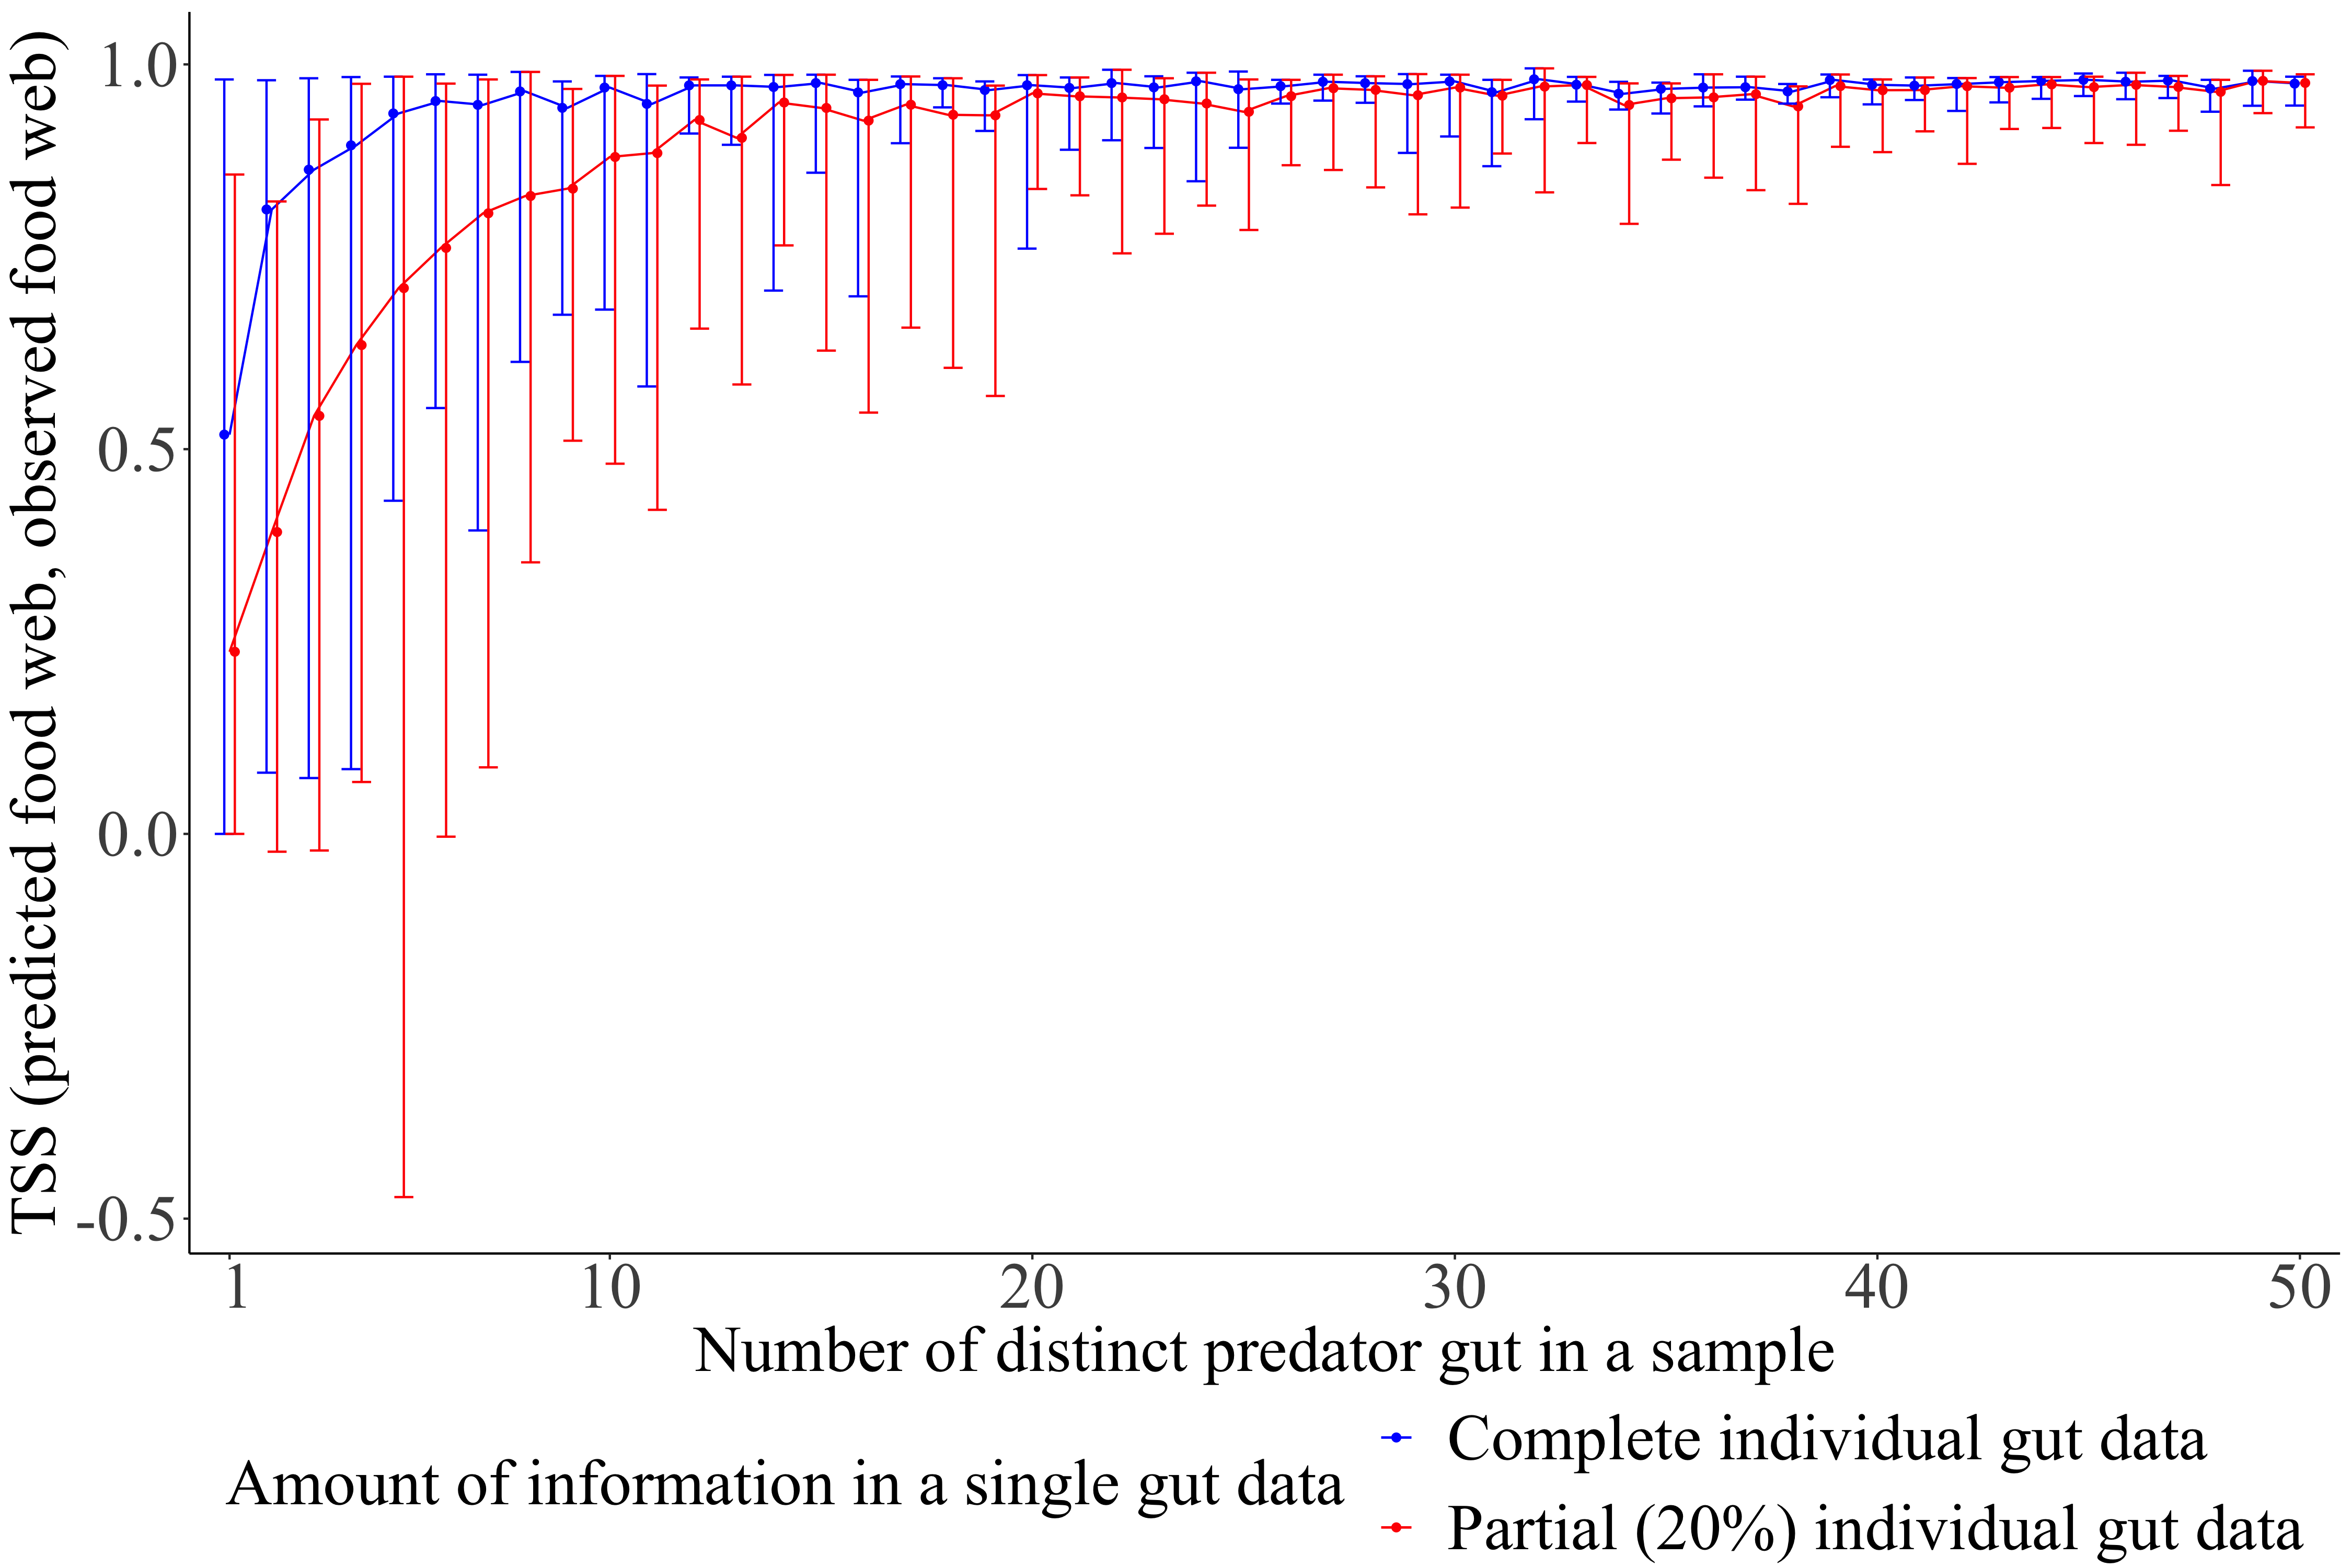
\includegraphics[width=400px]{../fig/TSS_with_n_pred_prop_simulated} 

}

\caption{\label{fig:fig_r0} True skill statistics between predicted food web and observed food web for a simulated small reef food web estimated for distinct predator guts in a sample. The observed simulated food web consists of 50 species and \dots links. The vertical bars correspond to the prediction intervals of the true skill statistics with filled circles representing the corresponding mean. A prediction interval of the TSS is formed using a set of 100 accepted TSS values using the ABC method.}\label{fig:fig_r0}
\end{figure}

The true skill statistics (TSS) between the predicted food web and
observed food web saturated with an increasing number of distinct
predator guts in a sample (Fig. \ref{fig:fig_r0}). The TSS of the
predicted food webs estimated using the complete individual gut data had
shorter prediction intervals resulting in less uncertainty, and higher
mean TSS than that using the partial individual gut data. The maximum
limit of the prediction interval of TSS estimated using the complete gut
data and the partial gut data were almost equal, with the minimum limit
of the prediction interval of TSS using partial gut data being lower
than that from the complete gut data. Eventually, the gap between the
mean TSS using the partial gut data and the complete gut data reduced
with an increasing number of distinct predator guts suggesting when we
have enough predator species' gut data, the achieved TSS was almost
constant and hence independent of the amount of gut data.

The maximum TSS estimated using the complete gut data was very close to
one and almost remained constant with an increasing number of different
predator species sampled. With the gut data sample of only five distinct
predator species, 95\% of the maximum mean TSS was achieved when
complete individual gut data was used, while the same was achieved with
15 predator species for partial gut data. This shows that one does not
need to know the gut data of all the species to predict the food web and
the accuracy is dependent on the completeness of an individual gut data.

\begin{figure}

{\centering 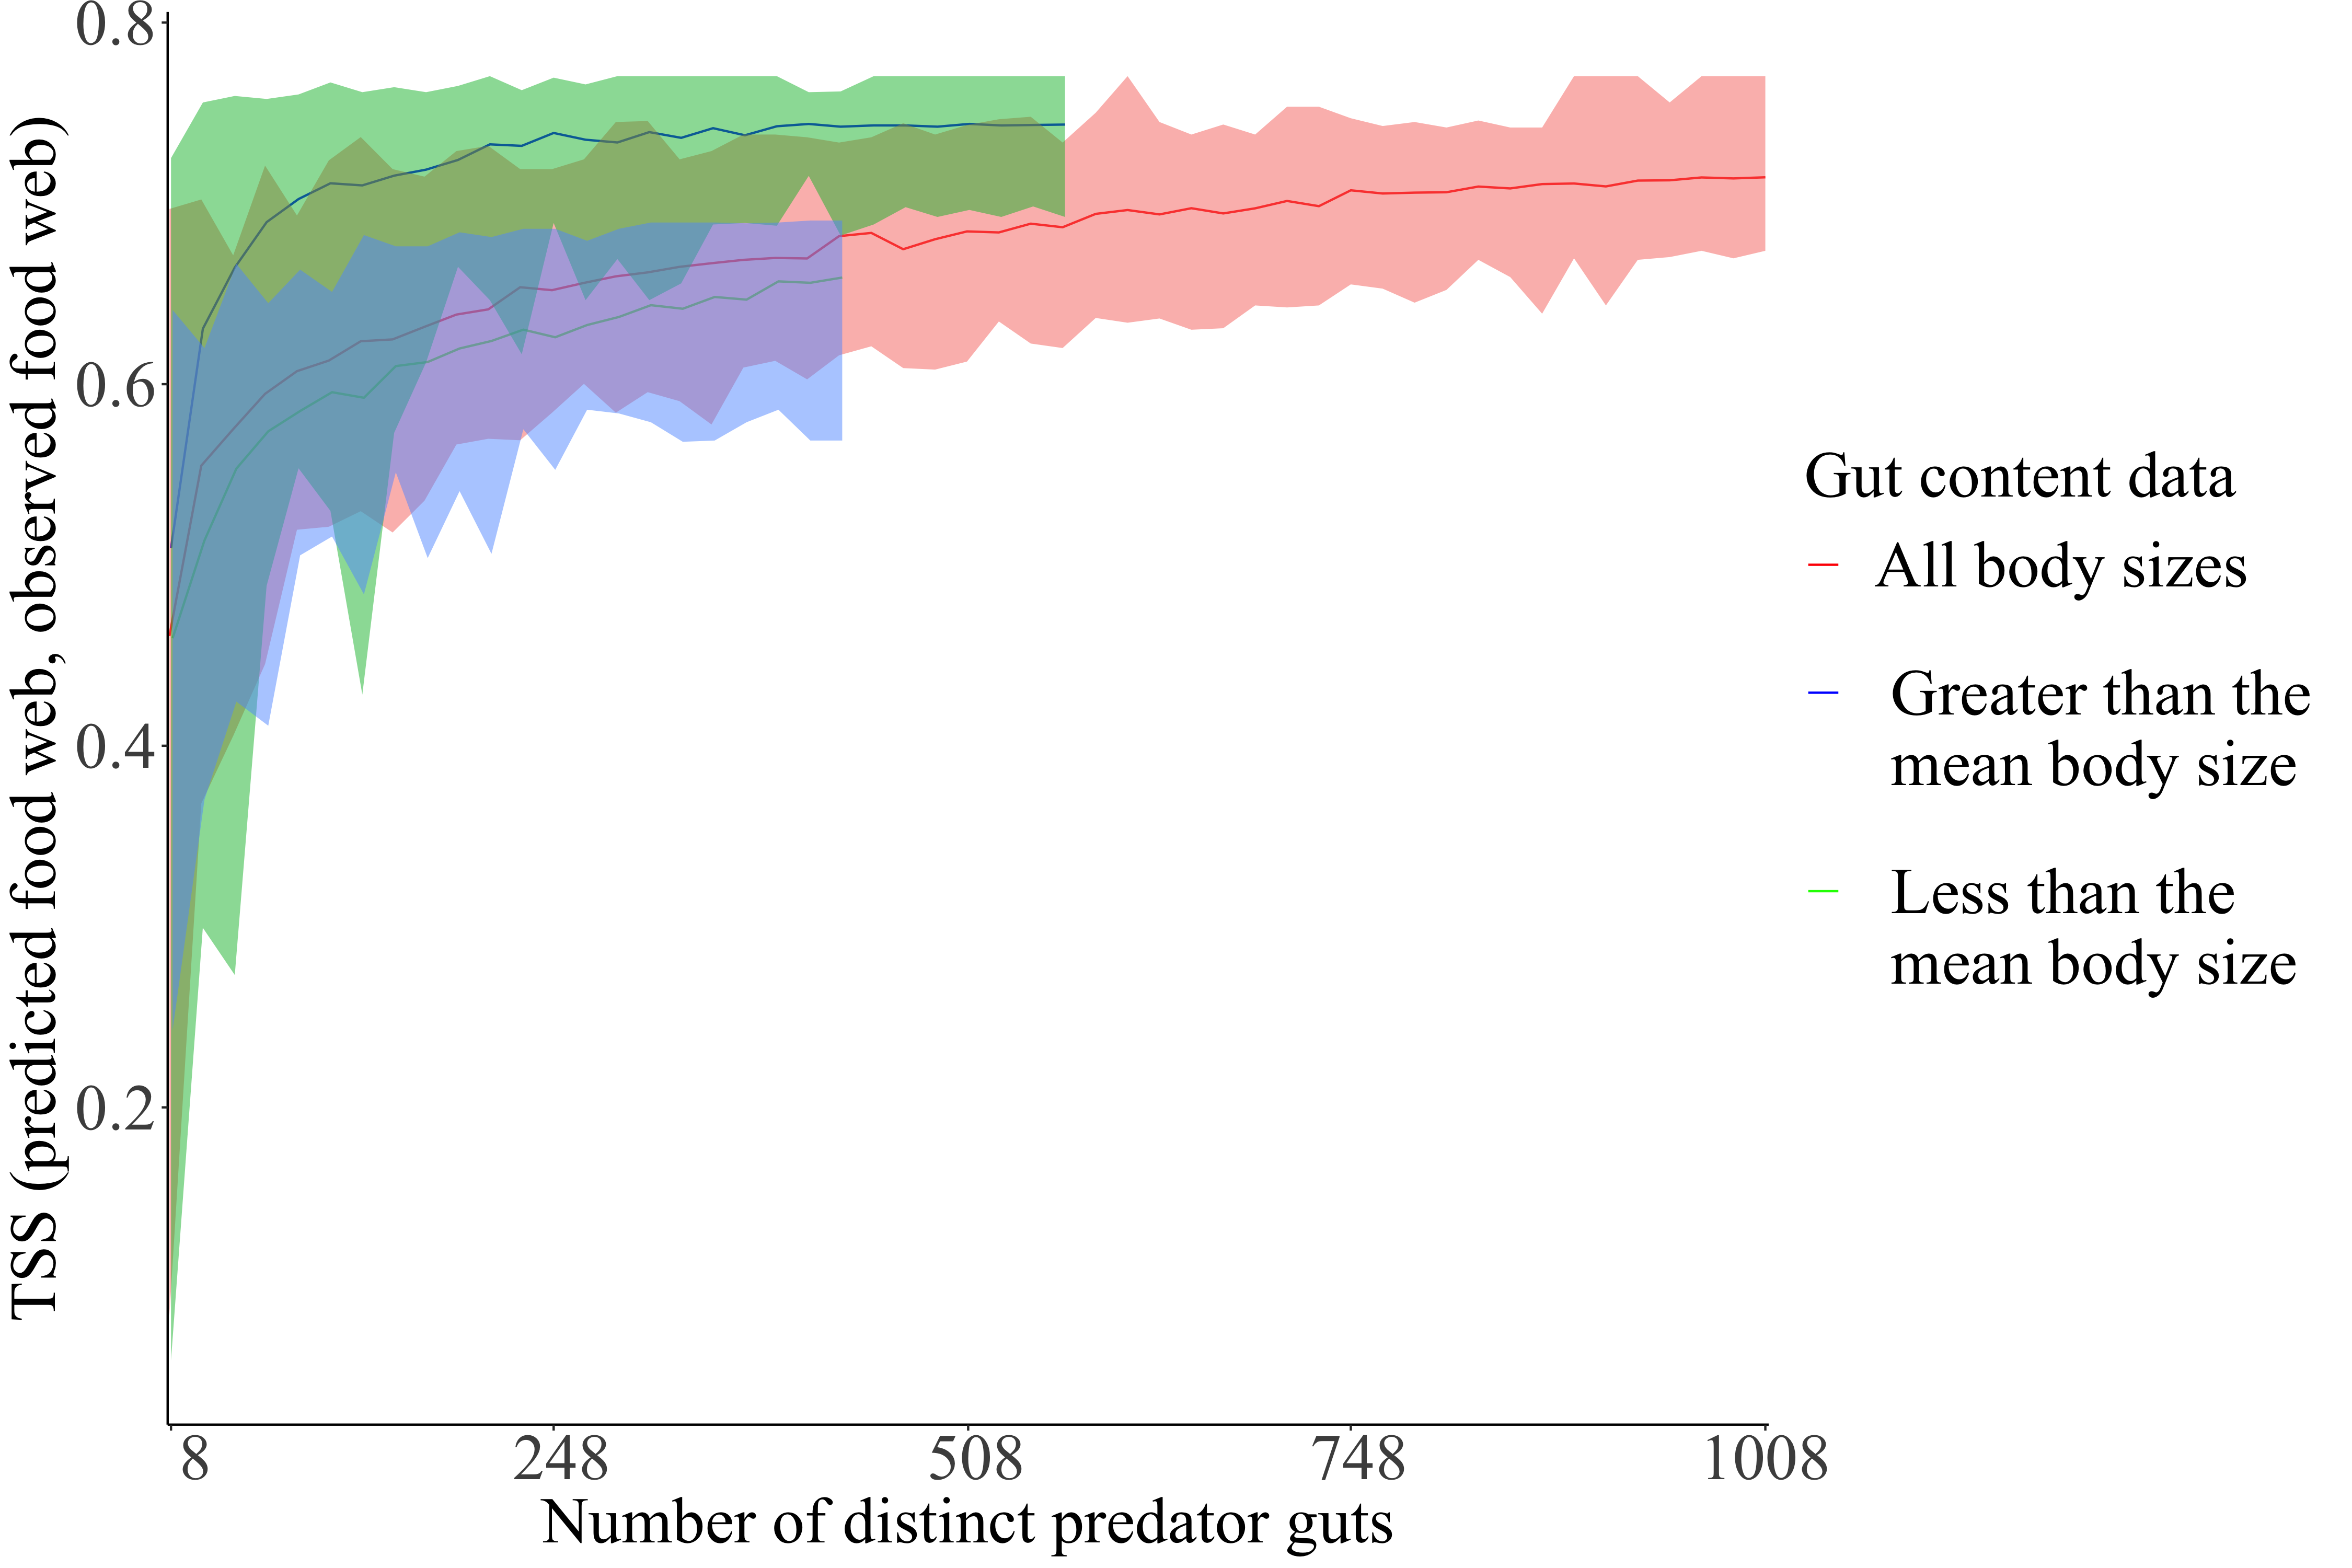
\includegraphics[width=300px]{../fig/TSS_with_n_pred_prop} 

}

\caption{\label{fig:fig_r3} True skill statistics between predicted food web and observed food web estimated for different number of distinct predator guts. The estimation is done for three sets of gut data: gut content data of predators whose body sizes are smaller than the mean body size, larger than the mean body size, and all the gut content data.}\label{fig:fig_r3}
\end{figure}

\begin{figure}

{\centering 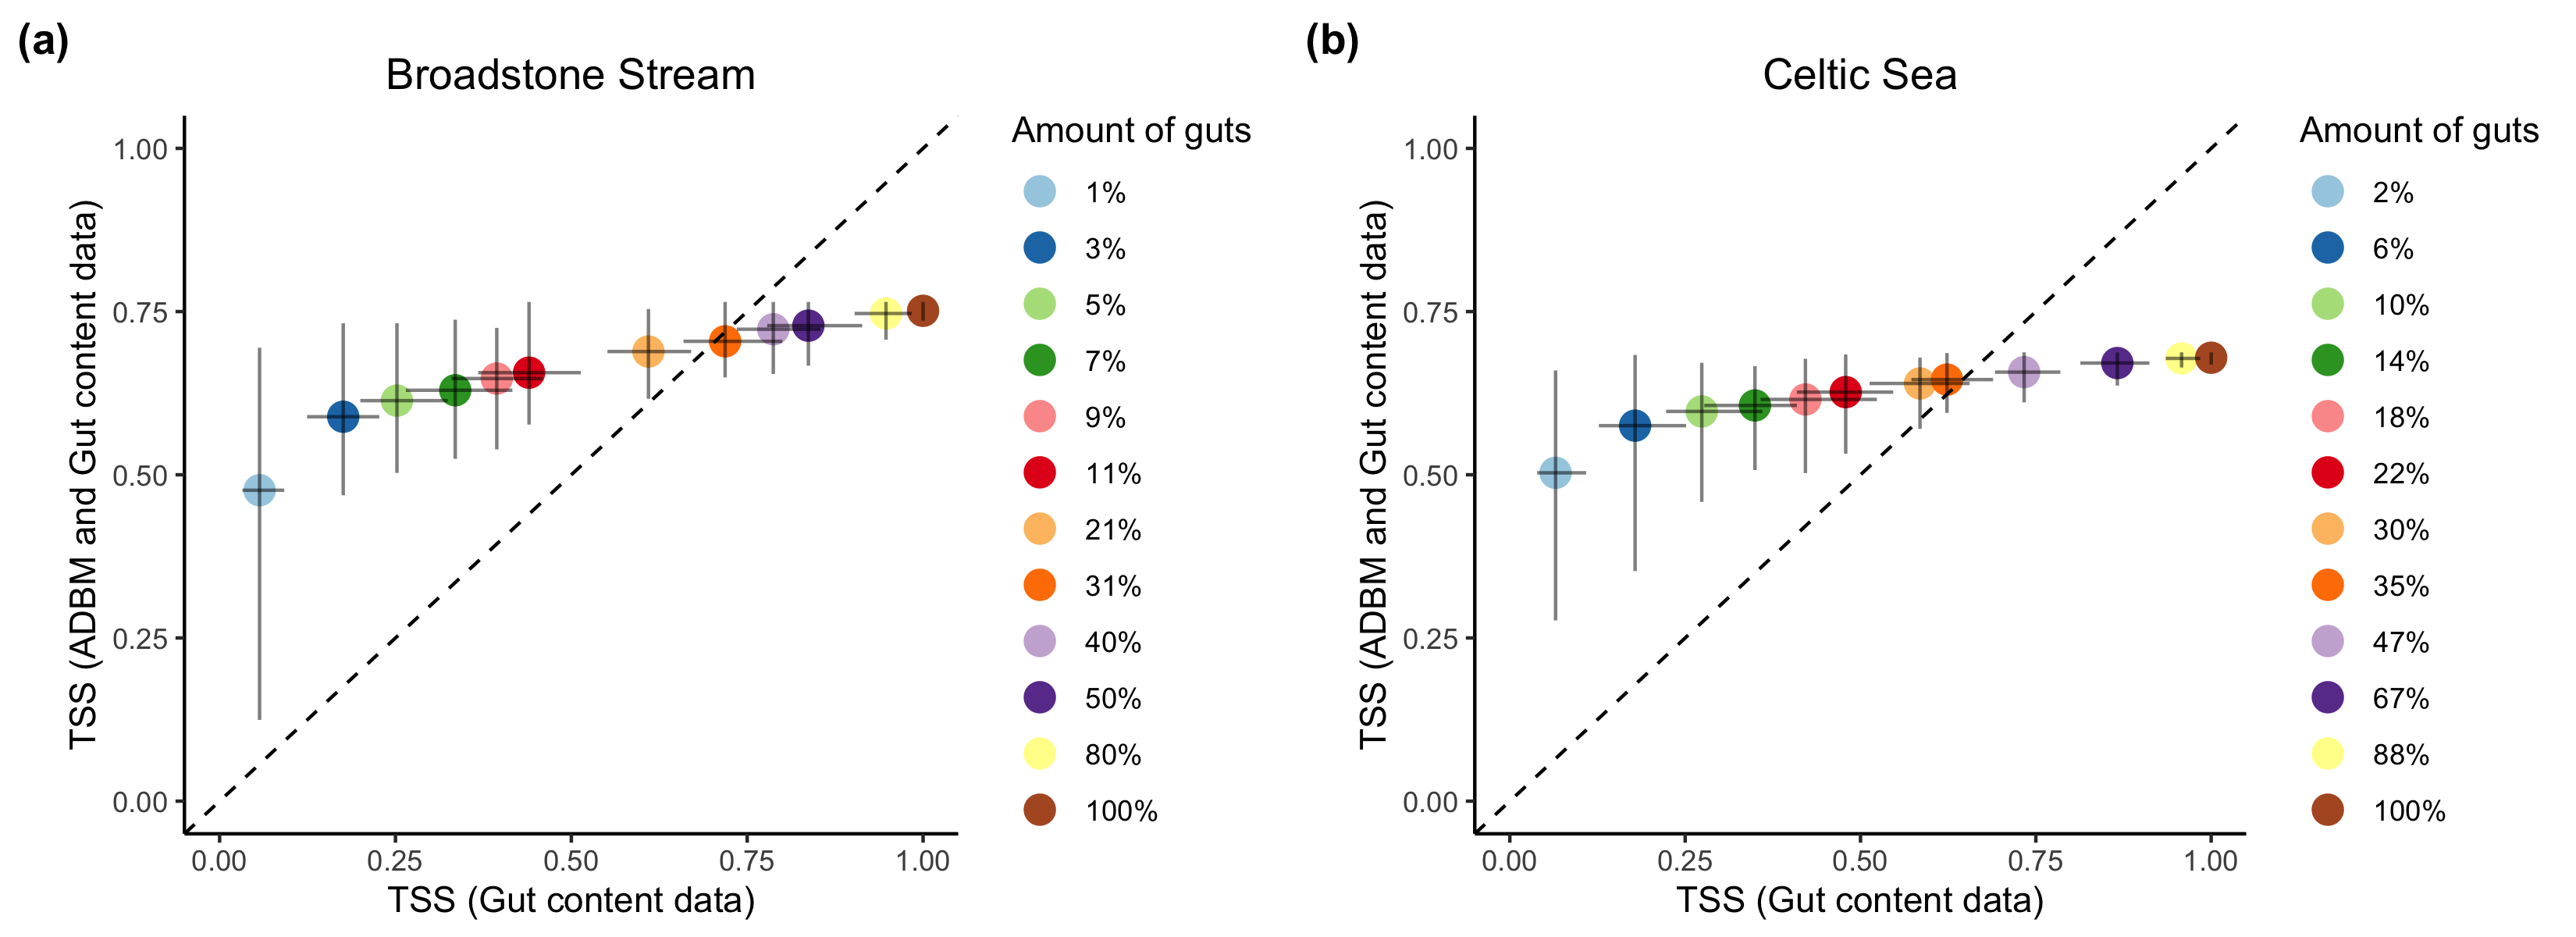
\includegraphics[width=500px]{../../results/misc/TSS_model_vs_data} 

}

\caption{\label{fig:fig_r31} True skill statistic between predicted food web using ADBM and incomplete gut content data, and observed food web against the true skill statistic between food web constructed using incomplete gut content data, and observed food web. Error bars represent prediction intervals of 100 independent samples. Dashed line is 1:1 line for reference.}\label{fig:fig_r31}
\end{figure}

\begin{figure}

{\centering 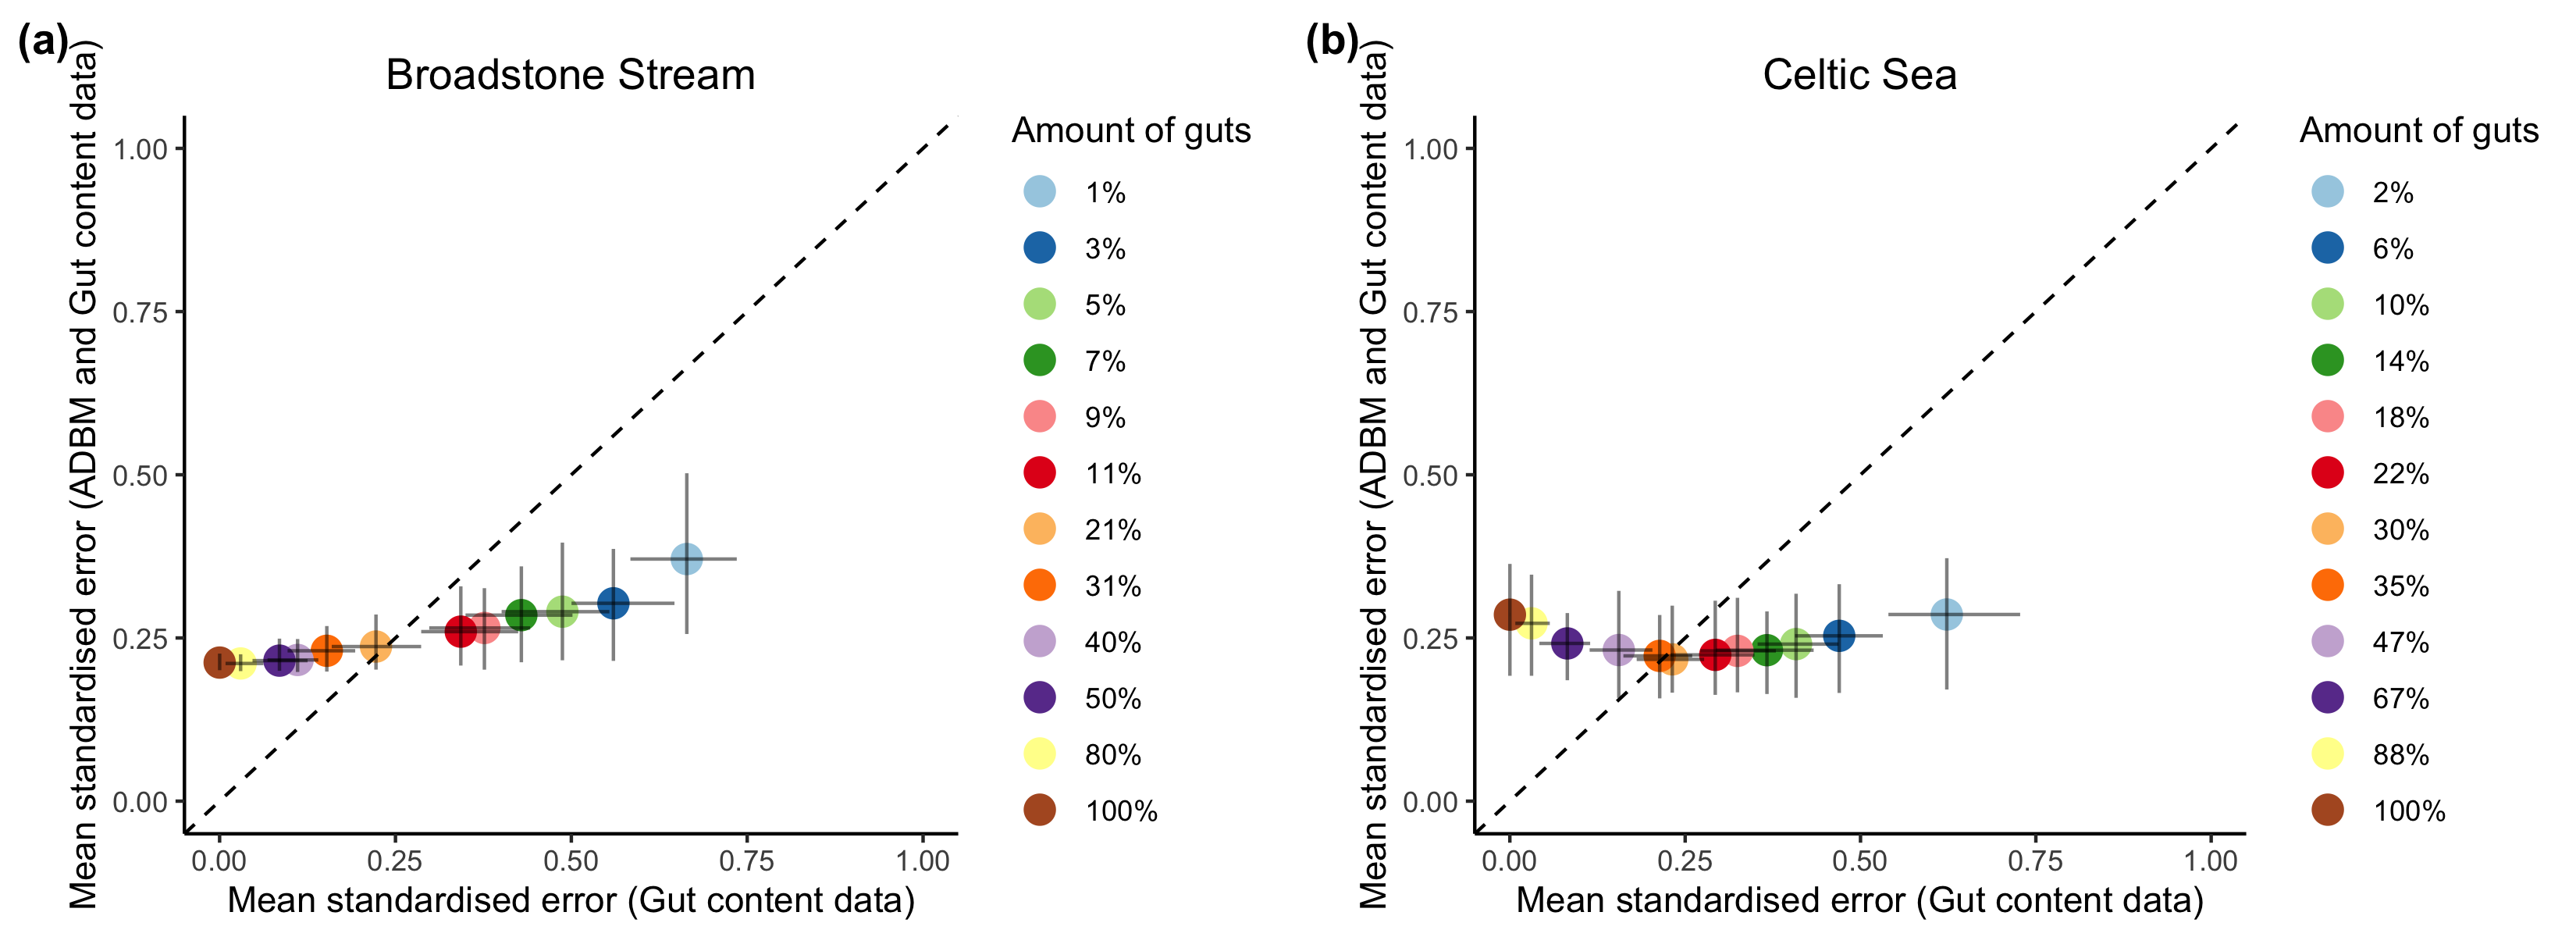
\includegraphics[width=500px]{../../results/misc/mse_model_vs_data} 

}

\caption{\label{fig:fig_r32} Mean standardised error in structural properties in the food web predicted using ADBM and incomplete gut content data against structural properties in the predicted food web constructed using incomplete gut content data. Error bars represent prediction intervals of 100 independent samples. Dashed line is 1:1 line for reference.}\label{fig:fig_r32}
\end{figure}

\hypertarget{acknowledgements}{%
\section{Acknowledgements}\label{acknowledgements}}

\hypertarget{author-contributions}{%
\section{Author contributions}\label{author-contributions}}

\hypertarget{references}{%
\section{References}\label{references}}

\hypertarget{refs}{}
\begin{CSLReferences}{1}{0}
\leavevmode\hypertarget{ref-allesinaGeneralModelFood2008}{}%
Allesina, Stefano, David Alonso, and Mercedes Pascual. 2008. {``A
{General Model} for {Food Web Structure}.''} \emph{Science} 320 (5876):
658--61. \url{https://doi.org/10.1126/science.1156269}.

\leavevmode\hypertarget{ref-alloucheAssessingAccuracySpecies2006}{}%
Allouche, Omri, Asaf Tsoar, and Ronen Kadmon. 2006. {``Assessing the
Accuracy of Species Distribution Models: Prevalence, Kappa and the True
Skill Statistic ({TSS}).''} \emph{Journal of Applied Ecology} 43 (6):
1223--32. \url{https://doi.org/10.1111/j.1365-2664.2006.01214.x}.

\leavevmode\hypertarget{ref-bakerFishGutContent2014}{}%
Baker, Ronald, Amanda Buckland, and Marcus Sheaves. 2014. {``Fish Gut
Content Analysis: Robust Measures of Diet Composition.''} \emph{Fish and
Fisheries} 15 (1): 170--77. \url{https://doi.org/10.1111/faf.12026}.

\leavevmode\hypertarget{ref-cohenSoilInvertebratesChemistry2014}{}%
Cohen, Joel E., and Christian Mulder. 2014. {``Soil Invertebrates,
Chemistry, Weather, Human Management, and Edaphic Food Webs at 135 Sites
in {The Netherlands}: {SIZEWEB}.''} \emph{Ecology} 95 (2): 578--78.
\url{https://doi.org/10.1890/13-1337.1}.

\leavevmode\hypertarget{ref-cohenStochasticTheoryCommunity1985}{}%
Cohen, Joel E., C. M. Newman, and John Hyslop Steele. 1985. {``A
Stochastic Theory of Community Food Webs {I}. {Models} and Aggregated
Data.''} \emph{Proceedings of the Royal Society of London. Series B.
Biological Sciences} 224 (1237): 421--48.
\url{https://doi.org/10.1098/rspb.1985.0042}.

\leavevmode\hypertarget{ref-crawfordApplicationsStableIsotope2008}{}%
Crawford, Kerry, Robbie A. Mcdonald, and Stuart Bearhop. 2008.
{``Applications of Stable Isotope Techniques to the Ecology of
Mammals.''} \emph{Mammal Review} 38 (1): 87--107.
\url{https://doi.org/10.1111/j.1365-2907.2008.00120.x}.

\leavevmode\hypertarget{ref-dixonAssessingDietNorth2017}{}%
Dixon, Heather J., J. Brian Dempson, Timothy F. Sheehan, Mark D.
Renkawitz, and Michael Power. 2017. {``Assessing the Diet of {North
American Atlantic} Salmon ({Salmo} Salar {L}.) Off the {West Greenland}
Coast Using Gut Content and Stable Isotope Analyses.''} \emph{Fisheries
Oceanography} 26 (5): 555--68. \url{https://doi.org/10.1111/fog.12216}.

\leavevmode\hypertarget{ref-dunneNetworkStructureBiodiversity2002}{}%
Dunne, Jennifer A., Richard J. Williams, and Neo D. Martinez. 2002.
{``Network Structure and Biodiversity Loss in Food Webs: Robustness
Increases with Connectance.''} \emph{Ecology Letters} 5 (4): 558--67.
\url{https://doi.org/10.1046/j.1461-0248.2002.00354.x}.

\leavevmode\hypertarget{ref-eitzingerTestingValidityFunctional2018}{}%
Eitzinger, Bernhard, Björn C. Rall, Michael Traugott, and Stefan Scheu.
2018. {``Testing the Validity of Functional Response Models Using
Molecular Gut Content Analysis for Prey Choice in Soil Predators.''}
\emph{Oikos} 127 (7): 915--26. \url{https://doi.org/10.1111/oik.04885}.

\leavevmode\hypertarget{ref-gilljamSeeingDouble2011}{}%
Gilljam, David, Aaron Thierry, Francois K. Edwards, David Figueroa,
Anton T. Ibbotson, J. Iwan Jones, Rasmus B. Lauridsen, Owen L. Petchey,
Guy Woodward, and Bo Ebenman. 2011. {``Seeing {Double}:''} In
\emph{Advances in {Ecological Research}}, 45:67--133. {Elsevier}.
\url{https://doi.org/10.1016/B978-0-12-386475-8.00003-4}.

\leavevmode\hypertarget{ref-goldwasserConstructionAnalysisLarge1993a}{}%
Goldwasser, Lloyd, and Jonathan Roughgarden. 1993. {``Construction and
{Analysis} of a {Large Caribbean Food Web}.''} \emph{Ecology} 74 (4):
1216--33. \url{https://doi.org/10.2307/1940492}.

\leavevmode\hypertarget{ref-gravelInferringFoodWeb2013}{}%
Gravel, Dominique, Timoth'ee Poisot, Camille Albouy, Laure Velez, and
David Mouillot. 2013. {``Inferring Food Web Structure from Predator-Prey
Body Size Relationships.''} Edited by Robert Freckleton. \emph{Methods
in Ecology and Evolution} 4 (11): 1083--90.
\url{https://doi.org/10.1111/2041-210X.12103}.

\leavevmode\hypertarget{ref-grayJoiningDotsAutomated2015}{}%
Gray, Clare, David H. Figueroa, Lawrence N. Hudson, Athen Ma, Dan
Perkins, and Guy Woodward. 2015. {``Joining the Dots: {An} Automated
Method for Constructing Food Webs from Compendia of Published
Interactions.''} \emph{Food Webs} 5 (December): 11--20.
\url{https://doi.org/10.1016/j.fooweb.2015.09.001}.

\leavevmode\hypertarget{ref-hattabForecastingFinescaleChanges2016}{}%
Hattab, Tarek, Fabien Leprieur, Frida Ben Rais Lasram, Dominique Gravel,
François Le Loc'h, and Camille Albouy. 2016. {``Forecasting Fine-Scale
Changes in the Food-Web Structure of Coastal Marine Communities Under
Climate Change.''} \emph{Ecography} 39 (12): 1227--37.
\url{https://doi.org/10.1111/ecog.01937}.

\leavevmode\hypertarget{ref-hildrewChapterSustainedResearch2009}{}%
Hildrew, Alan G. 2009. {``Chapter 4 {Sustained Research} on {Stream
Communities}.''} In \emph{Advances in {Ecological Research}},
41:175--312. {Elsevier}.
\url{https://doi.org/10.1016/S0065-2504(09)00404-8}.

\leavevmode\hypertarget{ref-hyslopStomachContentsAnalysis1980}{}%
Hyslop, E. J. 1980. {``Stomach Contents Analysis---a Review of Methods
and Their Application.''} \emph{Journal of Fish Biology} 17 (4):
411--29. \url{https://doi.org/10.1111/j.1095-8649.1980.tb02775.x}.

\leavevmode\hypertarget{ref-jordanKeystoneSpeciesFood2009}{}%
Jord'an, Ferenc. 2009. {``Keystone Species and Food Webs.''}
\emph{Philosophical Transactions of the Royal Society B: Biological
Sciences} 364 (1524): 1733--41.
\url{https://doi.org/10.1098/rstb.2008.0335}.

\leavevmode\hypertarget{ref-kadoyaIsoWebBayesianIsotope2012}{}%
Kadoya, Taku, Yutaka Osada, and Gaku Takimoto. 2012. {``{IsoWeb}: {A
Bayesian Isotope Mixing Model} for {Diet Analysis} of the {Whole Food
Web}.''} Edited by Simon Thrush. \emph{PLoS ONE} 7 (7): e41057.
\url{https://doi.org/10.1371/journal.pone.0041057}.

\leavevmode\hypertarget{ref-layerFoodWebStructure2010}{}%
Layer, Katrin, Jens O. Riede, Alan G. Hildrew, and Guy Woodward. 2010.
{``Food {Web Structure} and {Stability} in 20 {Streams Across} a {Wide
pH Gradient}.''} In \emph{Advances in {Ecological Research}},
42:265--99. {Elsevier}.
\url{https://doi.org/10.1016/B978-0-12-381363-3.00005-8}.

\leavevmode\hypertarget{ref-laymanCanStableIsotope2007}{}%
Layman, Craig A., D. Albrey Arrington, Carmen G. Montaña, and David M.
Post. 2007. {``Can {Stable Isotope Ratios Provide} for {Community}-{Wide
Measures} of {Trophic Structure}?''} \emph{Ecology} 88 (1): 42--48.
\url{https://doi.org/10.1890/0012-9658(2007)88\%5B42:CSIRPF\%5D2.0.CO;2}.

\leavevmode\hypertarget{ref-lindegrenEcologicalForecastingClimate2010}{}%
Lindegren, Martin, Christian Möllmann, Anders Nielsen, Keith Brander,
Brian R. MacKenzie, and Nils Chr. Stenseth. 2010. {``Ecological
Forecasting Under Climate Change: The Case of {Baltic} Cod.''}
\emph{Proceedings of the Royal Society B: Biological Sciences} 277
(1691): 2121--30. \url{https://doi.org/10.1098/rspb.2010.0353}.

\leavevmode\hypertarget{ref-macarthurOptimalUsePatchy1966}{}%
MacArthur, Robert H., and Eric R. Pianka. 1966. {``On {Optimal Use} of a
{Patchy Environment}.''} \emph{The American Naturalist} 100 (916):
603--9. \url{http://www.jstor.org/stable/2459298}.

\leavevmode\hypertarget{ref-mcclain-countsTrophicStructureMesopelagic2017b}{}%
McClain-Counts, Jennifer P., Amanda W. J. Demopoulos, and Steve W. Ross.
2017. {``Trophic Structure of Mesopelagic Fishes in the {Gulf} of
{Mexico} Revealed by Gut Content and Stable Isotope Analyses.''} Journal
Article. \emph{Marine Ecology} 38 (4).
\url{https://doi.org/10.1111/maec.12449}.

\leavevmode\hypertarget{ref-ogormanSimpleModelPredicts2019}{}%
O'NAGorman, Eoin J., Owen L. Petchey, Katy J. Faulkner, Bruno Gallo,
Timothy A. C. Gordon, Joana Neto-Cerejeira, J'on S. 'Olafsson, Doris E.
Pichler, Murray S. A. Thompson, and Guy Woodwar. 2019. {``A Simple Model
Predicts How Warming Simplifies Wild Food Webs.''} \emph{Nature Climate
Change} 9 (8, 8): 611--16.
\url{https://doi.org/10.1038/s41558-019-0513-x}.

\leavevmode\hypertarget{ref-omalleyEffectsFoodWeb2017}{}%
O'NAMalley, Brian P., Lars G. Rudstam, James M. Watkins, Toby J. Holda,
and Brian C. Weide. 2017. {``Effects of Food Web Changes on {Mysis}
Diluviana Diet in {Lake Ontario}.''} \emph{Journal of Great Lakes
Research}, Special {section} on {Lake Ontario CSMI} 2013, 43 (5):
813--22. \url{https://doi.org/10.1016/j.jglr.2017.02.003}.

\leavevmode\hypertarget{ref-peralta-maraverStructureDynamicsStability2017}{}%
Peralta-Maraver, I., M. J. Lopez-Rodriguez, and J. M. Tierno de
Figueroa. 2017. {``Structure, Dynamics and Stability of a
{Mediterranean} River Food Web.''} \emph{Marine and Freshwater Research}
68 (3): 484--95. \url{https://doi.org/10.1071/MF15154}.

\leavevmode\hypertarget{ref-petcheySizeForagingFood2008}{}%
Petchey, Owen L., Andrew P. Beckerman, Jens O. Riede, and Philip H.
Warren. 2008. {``Size, Foraging, and Food Web Structure.''}
\emph{Proceedings of the National Academy of Sciences} 105: 4191--96.
\url{https://doi.org/10.1073/pnas.0710672105}.

\leavevmode\hypertarget{ref-rindorfBiasEstimatingFood2004}{}%
Rindorf, A, and P Lewy. 2004. {``Bias in Estimating Food Consumption of
Fish by Stomach-Content Analysis''} 61: 12.

\leavevmode\hypertarget{ref-roslinUseDNABarcodes2016}{}%
Roslin, Tomas, and Sanna Majaneva. 2016. {``The Use of {DNA} Barcodes in
Food Web Construction---Terrestrial and Aquatic Ecologists Unite!''}
Edited by Elizabeth Clare. \emph{Genome} 59 (9): 603--28.
\url{https://doi.org/10.1139/gen-2015-0229}.

\leavevmode\hypertarget{ref-schmid-arayaImportanceMeiofaunaFood2002}{}%
Schmid-Araya, J. M., A. G. Hildrew, A. Robertson, P. E. Schmid, and J.
Winterbottom. 2002. {``The {Importance} of {Meiofauna} in {Food Webs}:
{Evidence} from an {Acid Stream}.''} \emph{Ecology} 83 (5): 1271--85.
\url{https://doi.org/10.1890/0012-9658(2002)083\%5B1271:TIOMIF\%5D2.0.CO;2}.

\leavevmode\hypertarget{ref-schmid-arayaConnectanceStreamFood2002}{}%
Schmid-Araya, Jenny M., Peter E. Schmid, Anne Robertson, Julie
Winterbottom, Charlotte Gjerløv, and Alan G. Hildrew. 2002.
{``Connectance in {Stream Food Webs}.''} \emph{Journal of Animal
Ecology} 71 (6): 1056--62. \url{http://www.jstor.org/stable/1555780}.

\leavevmode\hypertarget{ref-tamaddoni-nezhadConstructionValidationFood2013}{}%
Tamaddoni-Nezhad, Alireza, Ghazal Afroozi Milani, Alan Raybould, Stephen
Muggleton, and David A. Bohan. 2013. {``Construction and {Validation} of
{Food Webs Using Logic}-{Based Machine Learning} and {Text Mining}.''}
In \emph{Advances in {Ecological Research}}, 49:225--89. {Elsevier}.
\url{https://doi.org/10.1016/B978-0-12-420002-9.00004-4}.

\leavevmode\hypertarget{ref-warrenSpatialTemporalVariation1989}{}%
Warren, Philip H. 1989. {``Spatial and {Temporal Variation} in the
{Structure} of a {Freshwater Food Web}.''} \emph{Oikos} 55 (3): 299.
\url{https://doi.org/10.2307/3565588}.

\leavevmode\hypertarget{ref-woodwardIndividualBasedFoodWebs2010}{}%
Woodward, Guy, Julia Blanchard, Rasmus B. Lauridsen, Francois K.
Edwards, J. Iwan Jones, David Figueroa, Philip H. Warren, and Owen L.
Petchey. 2010. {``Individual-{Based Food Webs}.''} In \emph{Advances in
{Ecological Research}}, 43:211--66. {Elsevier}.
\url{https://doi.org/10.1016/B978-0-12-385005-8.00006-X}.

\leavevmode\hypertarget{ref-woodwardQuantificationResolutionComplex2005}{}%
Woodward, Guy, Dougie C. Speirs, and Alan G. Hildrew. 2005a.
{``Quantification and {Resolution} of a {Complex}, {Size}-{Structured
Food Web}.''} In \emph{Advances in {Ecological Research}}, 36:85--135.
{Elsevier}. \url{https://doi.org/10.1016/S0065-2504(05)36002-8}.

\leavevmode\hypertarget{ref-woodwardQuantificationResolutionComplex2005a}{}%
---------. 2005b. {``Quantification and {Resolution} of a {Complex},
{Size}-{Structured Food Web}.''} In \emph{Advances in {Ecological
Research}}, 36:85--135. {Elsevier}.
\url{https://doi.org/10.1016/S0065-2504(05)36002-8}.

\end{CSLReferences}

\bibliographystyle{unsrt}
\bibliography{bibliography.bib}


\end{document}
